\documentclass[11pt]{article}

\usepackage[a4paper,margin=1.2in]{geometry}
\usepackage{amsmath,amssymb,amsthm,mathtools}
\usepackage{xcolor}
\usepackage{hyperref}
\usepackage{booktabs}
\usepackage{array}
\usepackage{tabularx}
\usepackage{enumitem}
\usepackage{graphicx}
\usepackage{subcaption}
\usepackage{caption}
\graphicspath{{../figures/}{figures/}}

\hypersetup{colorlinks=true, linkcolor=blue!50!black, citecolor=blue!50!black}

\newtheorem{theorem}{Theorem}
\newtheorem{proposition}[theorem]{Proposition}
\newtheorem{lemma}[theorem]{Lemma}
\newtheorem{corollary}[theorem]{Corollary}
\theoremstyle{definition}
\newtheorem{definition}[theorem]{Definition}
\theoremstyle{remark}
\newtheorem{remark}[theorem]{Remark}
\theoremstyle{definition}
\newtheorem{assumption}{Assumption}

\newcommand{\E}{\mathbb{E}}
\newcommand{\Var}{\mathrm{Var}}
\newcommand{\Prob}{\mathbb{P}}
\newcommand{\R}{\mathbb{R}}
\newcommand{\VaR}{\mathrm{VaR}}
\newcommand{\ES}{\mathrm{ES}}
\newcommand{\GPD}{\mathrm{GPD}}
\newcommand{\NB}{\mathrm{NB}}
\newcommand{\TVL}{\mathrm{TVL}}
\newcommand{\1}{\mathbf{1}}
\newcolumntype{L}[1]{>{\raggedright\arraybackslash}p{#1}}

\title{Study Companion: \\
The Statistics and Economics of\\
\emph{Pricing the DeFi Tail:\\ Do Protocols or Depositors Price Operational Risk?}}
\author{Nils Bundi}
\date{}

\begin{document}
\maketitle
\tableofcontents
\vspace{1em}

\noindent\textit{This document is a step-by-step companion to the main paper.
Where the paper is terse, this document is verbose: it spells out the
statistics, provides intuition for each modeling choice, and connects the
derivations to standard results in extreme-value theory, actuarial risk
measurement, and the economics of market discipline. Read this side-by-side
with the paper.}

\bigskip
\hrule
\bigskip

% ===========================================================================
\section{The setup}\label{sec:setup}
% ===========================================================================

The setup has four pieces: the economic object (a DeFi ``earn'' product), the
risk being measured (operational risk, in the banking sense), the question
(who bears the tail and is it priced), and the yardstick (a Basel
loss-distribution approach). Each piece is a deliberate choice. This section
walks through every choice with its motivation.

\subsection{The economic object: an earn product}

DeFi offers yield-bearing \emph{earn products}: a lending-pool supply position,
a decentralized-exchange (DEX) liquidity-provision position, a yield vault, a
stablecoin LP position. Each pays a yield for supplying capital, and each is
presented to users as a low-risk place to park value. I hold one reference
point fixed throughout the paper, the \emph{bank deposit}, and read every earn
product against it. The introduction to the paper frames the comparison in three
beats, and this subsection walks through each and then expands.

\paragraph{Similar in one respect: exposure to operational risk.}
The paper's opening similarity claim is deliberately narrow. Similar to a bank
deposit, an earn product exposes its holder to \emph{operational risk}, the
losses from failed processes, people, systems, and external events
(Section~\ref{sec:oprisk} makes the Basel definition precise). In either product
the depositor hands over capital and holds a redeemable claim, and in both an
operational failure, a fraud, a system break, an external attack, can impair that
claim. That shared exposure is the entire point of comparison. The paper does
\emph{not} claim the two products are otherwise alike, and neither do I.

\paragraph{Unlike a bank: no regulated capital behind the claim.}
The decisive contrast is what stands behind the claim when an operational loss
occurs. A bank must hold operational-risk \emph{capital}, sized under Basel from
a \emph{loss-distribution approach} (LDA, Section~\ref{sec:lda}), so a regulated
buffer sits between a loss event and the depositor's claim. A DeFi protocol faces
no such requirement, and by default holds nothing. The two products therefore
expose the depositor to the same \emph{kind} of risk while placing opposite
amounts of capital behind the claim: alike in the exposure, opposite in the
protection.

\paragraph{The decentralisation illusion.}
It is tempting to think an earn product is \emph{safer} than a deposit, because
DeFi's architecture genuinely removes several risks that sit on a bank's balance
sheet. Smart-contract custody replaces the custodian, settlement is atomic, and
counterparty credit risk collapses into the overcollateralization embedded in the
contract. Aramonte et al.\ (2021) name the mistake the ``decentralisation
illusion.'' The risks DeFi removes are custody, settlement, and counterparty
credit. The risk it keeps, and in some cases concentrates, is \emph{operational}:
external attacks on contract code, insider-rugpull and internal-fraud events,
oracle and economic-design manipulation, configuration and deployment errors.
Removing the balance-sheet risks does nothing to the operational tail, and it is
exactly that tail this paper measures.

\paragraph{The decisive difference: who bears the residual.}
Put the three beats together. In banking an operational loss hits the bank's
capital first, and the depositor is further insulated by deposit insurance and a
resolution authority that can wind the bank down without touching an insured
claim. DeFi has none of this: no capital requirement, no deposit insurance, no
resolution authority. So the residual operational loss lands on the last
claimant, the depositor, not the protocol. The risk is \emph{transferred to the
depositor by construction}. That transfer is the pivot of the paper, and
Section~\ref{sec:question} develops the two responses that can absorb it.

\paragraph{Why the bank deposit is still the right benchmark (the expansion).}
Given that the two are opposite in protection, why measure one against the other
at all? Because the similarity that matters for a depositor is \emph{perceived}.
An earn product is marketed as a low-risk, yield-bearing place to park value, and
its mechanics, deposit, accrue yield, redeem, mimic a deposit closely enough that
an unsophisticated retail depositor, absent standardized risk disclosure, may
take it to be deposit-like and price it as if the same protections stood behind
it. The bank deposit is the benchmark the depositor \emph{implicitly assumes}, so
it is the right yardstick for asking whether the protection the depositor assumes
is the protection that is actually there. The gap between the two is the subject
of the whole paper.

\begin{remark}[Perceived deposit, not an equivalent one]
``Deposit-like'' throughout describes how an earn product is marketed and
perceived, not a claim that it carries the same risk as an insured, capitalized
bank deposit. It does not. The comparison is worth drawing precisely because the
perception and the protection diverge, and the size of that divergence is what
the paper quantifies.
\end{remark}

\paragraph{Why hold the methodology fixed and swap only the data?}
This is the paper's central rhetorical move. If I measure the DeFi tail with
\emph{exactly} the machinery Basel uses for banks (the loss-distribution
approach, Section~\ref{sec:lda}), then any difference in the conclusion is
attributable to DeFi, not to a different measuring stick. I do not pick a
favorable method; I inherit the supervisor's, so the comparison to a bank
deposit is made in the bank supervisor's own units.

\subsection{The risk: operational risk in the Basel sense}\label{sec:oprisk}

\begin{definition}[Operational risk]
The risk of loss resulting from inadequate or failed internal processes,
people and systems, or from external events. It \emph{excludes} market and
credit risk.
\end{definition}

Operational risk is the residual category --- fraud, system failure, execution
error, external attack. It is exactly the category DeFi cannot design away:
smart contracts remove custodial and counterparty-credit risk, but the code can
still be exploited, the team can still misconfigure an oracle, and the founder
can still rug the pool.

\paragraph{The Basel Level-1 taxonomy.}
Basel~II (BCBS d128, 2006) fixed a seven-category event-type taxonomy, carried
into the Basel~III finalization. I map five of them onto an autonomous
protocol; the two I omit --- Employment Practices and Damage to Physical
Assets --- have no on-chain analogue. The five that transfer:

\begin{center}
\small
\begin{tabular}{l L{3.5cm} L{6.6cm}}
\toprule
Code & Basel Level-1 & DeFi operational reading \\
\midrule
IF   & Internal Fraud & rugpull, owner-drain, insider exit-scam, malicious upgrade \\
EF   & External Fraud & contract bugs (reentrancy, access-control, rounding), key phishing, DNS hijack \\
CPBP & Clients, Products \& Business Practices & economic-design attacks: flashloan-governance, oracle/price manipulation, share-price inflation \\
BDSF & Business Disruption \& System Failures & chain-level: MEV, sequencer outage, chain halt \\
EDPM & Execution, Delivery \& Process Mgmt & team-side config/deployment errors: oracle mis-deployment, broken governance params \\
\bottomrule
\end{tabular}
\end{center}

\paragraph{Why the taxonomy is orthogonal to the DeFi sector.}
The DeFi \emph{sector} (Lending, DEX, Bridge, \dots) is the product's
\emph{economic function}. The Basel type is the \emph{failure mechanism}. They
are different axes, so crossing them is genuinely informative rather than
redundant. Empirically (paper Table~3) Bridge losses are almost pure EF (code
drains pooled collateral), while Lending and Stablecoin losses are mostly CPBP
(the economics were gamed, not the bytecode). Keep this orthogonality in mind:
it is why the paper fits \emph{per sector} rather than pooling
(Section~\ref{sec:persector}).

\subsection{The question: who bears the tail, and is it priced?}\label{sec:question}

\begin{remark}[The pivot of the whole paper]
In banking, a loss hits the bank's capital first, and the depositor is further
insulated by deposit insurance and a resolution authority. In DeFi there is no
insurance and no resolution authority, so the loss lands on the last claimant
--- the depositor. The residual risk is \emph{transferred to the depositor by
construction}.
\end{remark}

Given that, only two things can absorb the tail, and the paper is organized
around them as \emph{competing responses by different participants}.

\paragraph{Response 1: the protocol holds a capital buffer.}
Some protocols keep governance-owned on-chain reserves that perform the
function Basel calls capital: Aave's Umbrella safety module, the Sky (formerly
MakerDAO) surplus buffer, Compound's per-market reserve factor. No regulation
requires this, and the buffers that exist are sized by governance vote, not by
any loss model.

\paragraph{Response 2: the depositor demands a risk premium in the yield.}
Where the protocol holds no buffer, the depositor should require a supply yield
above the risk-free rate, sized to the tail they bear. This is the classic
\emph{market-discipline} mechanism by which uninsured bank creditors price
institutional risk into the yields they demand (Flannery 1998; Egan,
Horta\c{c}su \& Matvos 2017).

\paragraph{Why the two responses are substitutes.}
This is the conceptual key to Section~\ref{sec:responses}. A buffer and a yield
premium fund the \emph{same} tail from two sides. If the protocol pre-funds
with a buffer, the depositor needs less compensation; if it holds nothing, the
depositor should demand more. Egan et al.\ (2017) prove exactly this for banks
--- deposit rates and capital are jointly determined substitutes. So an
efficient DeFi market should show a \emph{negative} relationship between buffer
coverage and yield premium. That prediction is what the Mann--Whitney test in
Section~\ref{sec:mwtest} checks.

\subsection{The yardstick: a loss-distribution approach}

The measurement tool is the standard operational-risk \emph{loss-distribution
approach} (LDA), the same one a bank supervisor applies under Basel. I develop
it in full in Section~\ref{sec:lda}. For now, note only its shape: it turns a list of
event losses into an annual-loss distribution, and reads a capital number off
that distribution's tail. Because the tail of the annual loss is driven almost
entirely by the tail of a \emph{single} event's severity, the whole
construction stands or falls on estimating one number well --- the tail index
$\xi$ (Section~\ref{sec:xi}).

% ===========================================================================
\section{The dataset and the Basel tagging}\label{sec:data}
% ===========================================================================

A tail fit is only as good as its tail observations, so the data construction
is methodologically central, not preliminary bookkeeping.

\subsection{Why seven sources}

Every prior DeFi/crypto-loss study leans on \emph{one} feed, each with coverage
gaps. Tail estimation is maximally sensitive to \emph{missing large events}, so
the paper merges seven public feeds: DefiLlama, rekt.news, DeFiHackLabs,
kismp123 DSI, BlockSec, de.fi/rekt-database (4{,}030 records), and SlowMist
(2{,}100 records). The last two are broad and noisy --- they include memecoin
honeypots, CEX failures, individual phishing --- which is why the filter below
matters.

\subsection{Step 1: normalize and deduplicate}

The same event appears in several feeds under different names, so naive
concatenation double-counts. I deduplicate in two passes.

\paragraph{Pass A --- name clustering.}
Cluster records whose names match (fuzzily) within a 14-day window.

\paragraph{Pass B --- date-and-amount.}
Match records on the same date ($\pm 7$~days) \emph{and} loss within $\pm 10\%$.
This second pass catches \emph{cross-named} duplicates that Pass~A misses ---
the canonical example is ``Ronin Bridge'' versus ``Ronin Network,'' the same
USD~624~m event under two names.

\paragraph{Reconciling disagreeing amounts.}
When several sources report the same event with different dollar figures, the
reconciled loss is the \emph{median} of per-source amounts. Median, not mean,
is deliberate: it is robust to a single feed's outlier misreport. Because one
inflated figure sits in the tail --- exactly where the estimate is most
sensitive --- a mean would let a lone bad number distort $\xi$.

\subsection{Step 2: filter to DeFi operational risk}

Two filters keep only losses that are (a) on a DeFi \emph{protocol} and (b)
\emph{operational}. A regex over event names removes CEX events,
custodial-wallet failures, Ponzis, unattributed phishing, and wallet-software
exploits; a sector-gated second pass drops NFT-mint, memecoin, gambling,
GameFi, and trading-bot records.

\subsection{Step 3: infer sector and Basel type}

\paragraph{Sector inference.}
Each event is assigned one of seven sub-sectors (Bridge, Lending, DEX, Yield,
Stablecoin, Derivatives, Other). I use DefiLlama's category where present,
else a regex chain that resolves \emph{Bridge first} (it is the most distinct
and most consequential), then Lending, DEX, Stablecoin, Yield, Derivatives.

\paragraph{Risk-category (Basel) inference.}
Textual evidence (technique, description, name) is applied \emph{first}, with
DefiLlama's generic classification only as a fallback, so an operational
signature overrides a lazy label. The worked example is the February~2026
Moonwell cbETH event: an oracle priced collateral at USD~1.12 instead of
$\approx$~USD~2{,}200, and liquidation bots seized USD~1.78~m within minutes.
The root cause was an oracle \emph{mis-deployment} --- a team-side error ---
so it is tagged EDPM, not EF (which would be a code exploit).

\paragraph{Why inferential tagging is defensible, and its risk.}
Tagging by inference is a judgment layer and a possible source of bias. The
defense is transparency (the rules are stated, the code is released) plus the
orthogonality check of Table~3. The honest caveat --- and a good referee
question --- is how sensitive the per-sector $\xi$ estimates are to
reclassifying borderline events.

\subsection{Coverage and the final sample}

Restricting to events dated between 2020-01-01 (when DeFi first reached
material scale) and the 2026-05-29 data cutoff gives a
\emph{1{,}317-event consolidated sample} (USD~10.84~B) over
2020-02-11 to 2026-05-29. Two audit layers, now folded into the
consolidation pipeline, refine this to the working sample used for every
headline number:

\begin{enumerate}[leftmargin=1.4em]
\item A \emph{seven-agent sector re-audit} (one parallel pass per sector,
stored in \texttt{mistags.json}) reclassifies $277$ mistagged events:
OHM-fork reserve-currency losses are moved to Stablecoin, and
memecoin/launchpad/gaming/NFT/CEX reassignments are marked \texttt{NOT\_DEFI}.
The resulting $153$ non-DeFi records are dropped during consolidation, so
they never enter the dataset --- leaving a \emph{1{,}164-event DeFi dataset}.

\item A \emph{depositor-facing rule filter} (rules R1--R6 covering
governance-token dilution, borrower over-liquidation, treasury drains,
router-approval hijacks, frontend/DNS hijacks, and individual-wallet
phishing), applied when the DeFi dataset is loaded, drops the $89$ events
whose losses did not hit the sector's earn user (LP, supplier, holder).
\end{enumerate}

\noindent The result is the working sample of \emph{1{,}075 events} and
\emph{USD~9.45~B}. Roughly
half ($536$ of $1{,}075$) carry cross-source confirmation, and across those
the median loss-amount disagreement is only $1.9\%$. ``Gross'' means before
any funds returned --- a conservative choice, since netting recoveries would
only lower every downstream number.

\begin{assumption}[Gross loss and reporting completeness]\label{as:gross}
Losses are measured gross of funds later returned, and the feeds capture the
events that drive the tail. Under-reported small events bias the body of the
severity distribution downward but leave the large tail events, which set the
capital figures, intact.
\end{assumption}

\noindent Assumption~\ref{as:gross} makes the estimates conservative in a signed
way. Netting recoveries (about $6\%$ of the aggregate) would lower every
downstream number, and any missed small events would only lighten the body.
Neither direction can inflate the tail-driven capital figure, so the reported
numbers are, if biased, biased low.

% ===========================================================================
\section{The loss-distribution approach}\label{sec:lda}
% ===========================================================================

This is the statistical core. The LDA has three parts --- severity, frequency,
and their compound aggregation --- and one summary statistic (a tail risk
measure). I build each in turn, then assemble.

\subsection{Statement}

For each sector I model the annual aggregate operational loss as a random sum
\begin{equation}\label{eq:compound}
S \;=\; \sum_{i=1}^{N} X_i,
\qquad N \sim \NB(\hat\lambda,\hat\alpha),
\qquad X_i \overset{\text{iid}}{\sim} F_X,
\end{equation}
where $N$ (the number of events in a year) is drawn from a negative-binomial
\emph{frequency} model, each $X_i$ (a single event's loss) is drawn from a
\emph{severity} distribution $F_X$, and the two are independent. The capital
number is the $99.9\%$ quantile of $S$, and the pure premium is its mean:
\[
\text{capital} \;=\; \VaR_{99.9}(S), \qquad
\text{pure premium} \;=\; \E[S].
\]

The random sum in~\eqref{eq:compound} is the classical actuarial
collective-risk model, and it rests on three structural conditions worth
stating explicitly because everything downstream inherits them.

\begin{assumption}[Compound structure]\label{as:compound}
Within a sector, the single-event severities $X_1,X_2,\dots$ are independent and
identically distributed draws from one severity law $F_X$; the annual count $N$
is independent of the severities; and events do not influence one another's
size or timing.
\end{assumption}

\noindent What Assumption~\ref{as:compound} buys is tractability: the mean,
variance, and tail of $S$ then follow from $F_X$ and the count law alone,
without a joint model. What it costs is realism on two fronts I return to.
Severities are not truly identical across protocols of very different size
(Assumption~\ref{as:homogeneity}), and events are not truly independent in time
(Assumption~\ref{as:independence}). Both cost-directions are signed later, so
the reader can see which way each pushes the capital number.

\begin{remark}[Why the tail of $S$ is really the tail of one $X$]
Operational-loss severities are \emph{subexponential} (Section~\ref{sec:subexp}): a
large annual total is one catastrophic event, not an accumulation of moderate
ones. So $\VaR_{99.9}(S)$ is governed by the far tail of $F_X$, and estimating
that tail well is the whole game. This is why I spend most of my effort on
severity.
\end{remark}

\subsection{Step 1: severity by peaks-over-threshold}\label{sec:severity}

I treat individual gross losses as iid draws from $F_X$ and model only its
\emph{upper tail} parametrically, splicing an empirical body to a
generalized-Pareto tail.

\paragraph{Why model only the tail, and why a GPD?}
The Pickands--Balkema--de~Haan theorem is the tail analogue of the central
limit theorem. It says that for a very broad class of distributions, the excess
over a high threshold $u$,
\[
Y \;=\; X - u \mid X > u,
\]
converges as $u \to \infty$ to a \emph{generalized Pareto distribution} (GPD),
\emph{regardless} of the original $F_X$. So the theory tells me the shape to
fit above $u$ --- it is GPD --- and I need not commit to a parametric family
for the messy body, where data are dense and I simply resample empirically.

\begin{assumption}[GPD tail]\label{as:tail}
Above the selected threshold $u$, the exceedances $X-u\mid X>u$ are exactly
generalized-Pareto. This is the finite-$u$ version of the
Pickands--Balkema--de~Haan limit, and it is what licenses the parametric tail
fit while leaving the body non-parametric.
\end{assumption}

\noindent Assumption~\ref{as:tail} is not taken on faith. The mean-excess plot
(Figure~\ref{fig:meanexcess}), the QQ plots (Figure~\ref{fig:qqpanel}), and the
Kolmogorov--Smirnov distances all test it directly, and all three are consistent
with it in every sector (Section~\ref{sec:empirical}). The residual risk is that
$u$ is finite, so the limit is an approximation; the threshold-stability scan
(Figure~\ref{fig:threshstab}) is the guard against picking a $u$ where that
approximation has not yet taken hold.

\paragraph{The GPD.}
With shape $\xi$ and scale $\beta$, the excess distribution has density and
survival function
\[
g_{\xi,\beta}(y) = \frac{1}{\beta}\Bigl(1+\xi\tfrac{y}{\beta}\Bigr)^{-(1/\xi+1)},
\qquad
\bar G_{\xi,\beta}(y) = \Bigl(1+\xi\tfrac{y}{\beta}\Bigr)^{-1/\xi},
\qquad y>0.
\]
The paper reports the density; the survival function is the more intuitive
object for a tail. The two parameters carry very different information: $\beta$
is a \emph{scale} (the size of a typical excess, in USD~m), while $\xi$ is the
\emph{shape} --- how fast the tail decays --- and is the single most important
number in the paper (Section~\ref{sec:xi}).

\paragraph{Estimation: maximum likelihood.}
Given exceedances $y_1,\dots,y_{n_u}$, the GPD log-likelihood is
\begin{equation}\label{eq:gpdll}
\ell(\xi,\beta) \;=\; -\,n_u\log\beta
\;-\;\Bigl(\tfrac{1}{\xi}+1\Bigr)\sum_{i=1}^{n_u}\log\!\Bigl(1+\xi\tfrac{y_i}{\beta}\Bigr).
\end{equation}
There is no closed-form maximizer, so I optimize numerically with
\emph{multi-start Nelder--Mead}. Nelder--Mead is a derivative-free simplex
method, robust when the surface is awkward (GPD likelihoods can be flat or have
boundary issues near $\xi=0$); multi-start means I launch from several initial
points and keep the best maximizer, because heavy-tailed likelihoods are
notoriously multi-modal.

\subsection{Step 2: choosing the threshold $u$}\label{sec:threshold}

Choosing $u$ is \emph{the} practitioner problem in POT, and it is a
bias--variance tradeoff.

\paragraph{The tradeoff, concretely.}
Set $u$ too low and you admit body observations that are not yet GPD-distributed
--- that is \emph{bias}. Set $u$ too high and you keep too few exceedances
$n_u$, so $\hat\xi$ swings wildly from sample noise --- that is \emph{variance}.
The right $u$ is the lowest one at which the GPD approximation has ``kicked
in.''

\paragraph{The plateau-stability rule.}
I scan the quantile grid $\mathcal{Q}=\{0.50,0.55,\dots,0.90\}$ and take the
\emph{highest} $q$ at which $\hat\xi(q)$ has stopped moving --- stable to within
$\tau=0.30$ as the threshold rises (the ``plateau'' in a threshold-stability
plot). Two practitioner floors guard the exceedance count: $n_u\ge 20$
(Embrechts, Kl\"uppelberg \& Mikosch 1997) and $n_u/n\ge 10\%$ (DuMouchel's
1983 ``top 10\%'' rule). If no $q$ satisfies the plateau, I fall back to the
lowest eligible quantile. The point is a \emph{rule-based, reproducible}
threshold: hand-picking $u$ is the classic way to engineer a tail estimate.

\paragraph{The mean-excess diagnostic.}
The visual companion is the mean-excess plot. For a GPD the mean-excess function
is \emph{linear} in $u$,
\[
e(u) \;=\; \E[X-u \mid X>u] \;=\; \frac{\beta+\xi(u-u_0)}{1-\xi}
\qquad (\xi<1),
\]
with slope $\xi/(1-\xi)$. So an upward-sloping straight mean-excess plot above
some $u$ is a signature of a GPD tail, and its slope already tells you the sign
and rough size of $\xi$. Figure~\ref{fig:meanexcess} plots $e(u)$ per sector on
log-log axes. Every sector's curve is monotonically increasing and near-linear
across two decades of threshold, which is precisely the visual signature of a
Pareto-type ($\xi>0$) tail. Bridge sits an order of magnitude above the other
curves, the first visible sign of the heavy tail the POT-GPD fit later pins at
$\hat\xi=1.74$. The diagnostic matters because it is model-free: it certifies a
GPD-shaped tail before any GPD is fitted, so the later parametric fit is
confirming a shape the data already show rather than imposing one.

\begin{figure}[t]
\centering
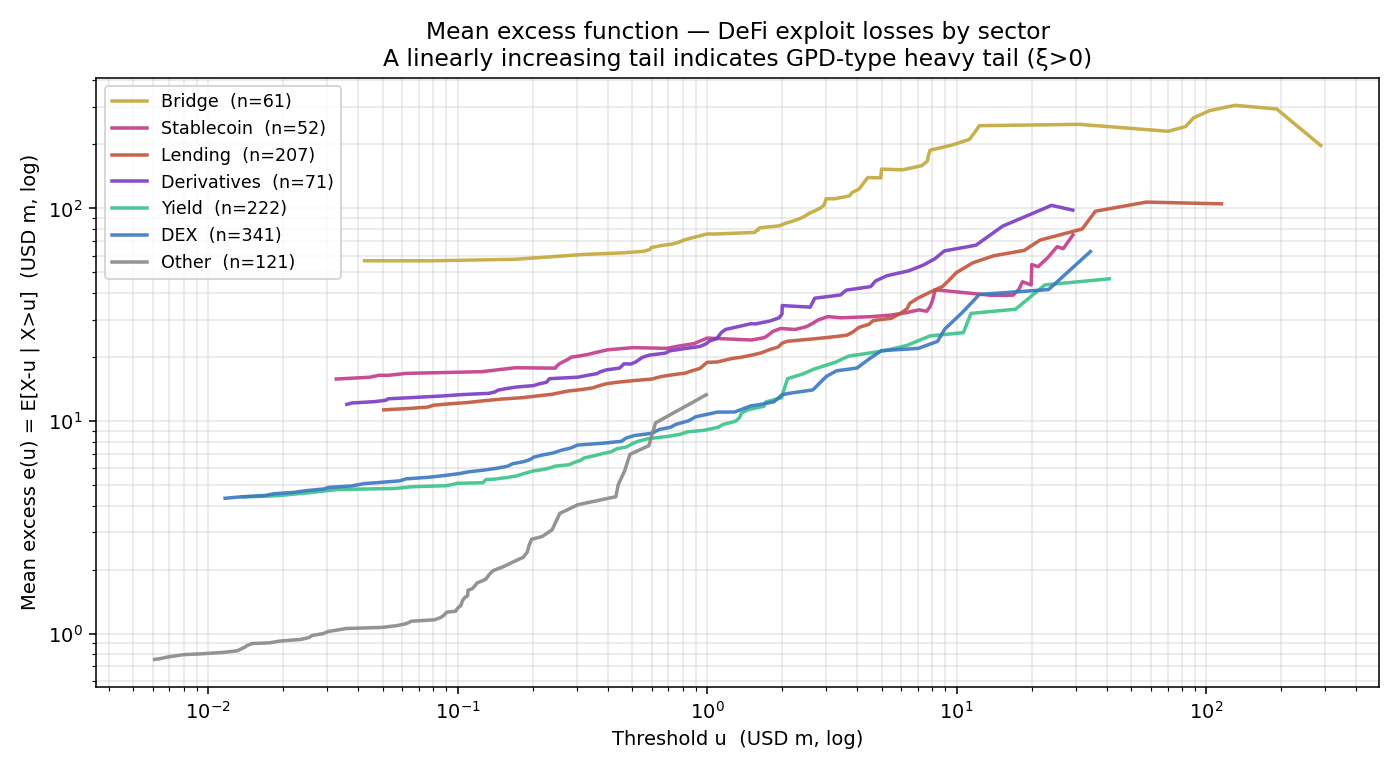
\includegraphics[width=0.86\linewidth]{r1_mean_excess.png}
\caption{Mean-excess function $e(u)=\E[X-u\mid X>u]$ per sector (log-log axes).
An approximately linear, upward-sloping curve is the signature of a
generalized-Pareto ($\xi>0$) tail. All seven sectors satisfy it across two
decades of threshold; Bridge is offset upward by its six nine-figure
mega-events, foreshadowing the heaviest $\hat\xi$.}
\label{fig:meanexcess}
\end{figure}

\paragraph{The Hill cross-check.}
The Hill estimator is a second, semi-parametric tail-index estimator that uses
only the top $k+1$ order statistics and makes no threshold choice beyond $k$. It
is an independent route to $\xi$, so agreement between the Hill plot and the
POT-GPD fit is genuine corroboration rather than the same estimator twice.
Figure~\ref{fig:hill} plots $\hat\xi_H(k)$ per sector against the two reference
lines that organize the whole paper: $\xi=1$ (the infinite-mean boundary) and
$\xi=0.5$ (the infinite-variance boundary). Bridge plateaus in the band
$[1.2,2.5]$, above the infinite-mean line, while every other sector plateaus in
$[0.4,1.0]$ below it. This is the same finite-mean-versus-infinite-mean split
the POT-GPD fits deliver, reached by a different estimator, which is why the two
diagnostics together make the split credible.

\begin{figure}[t]
\centering
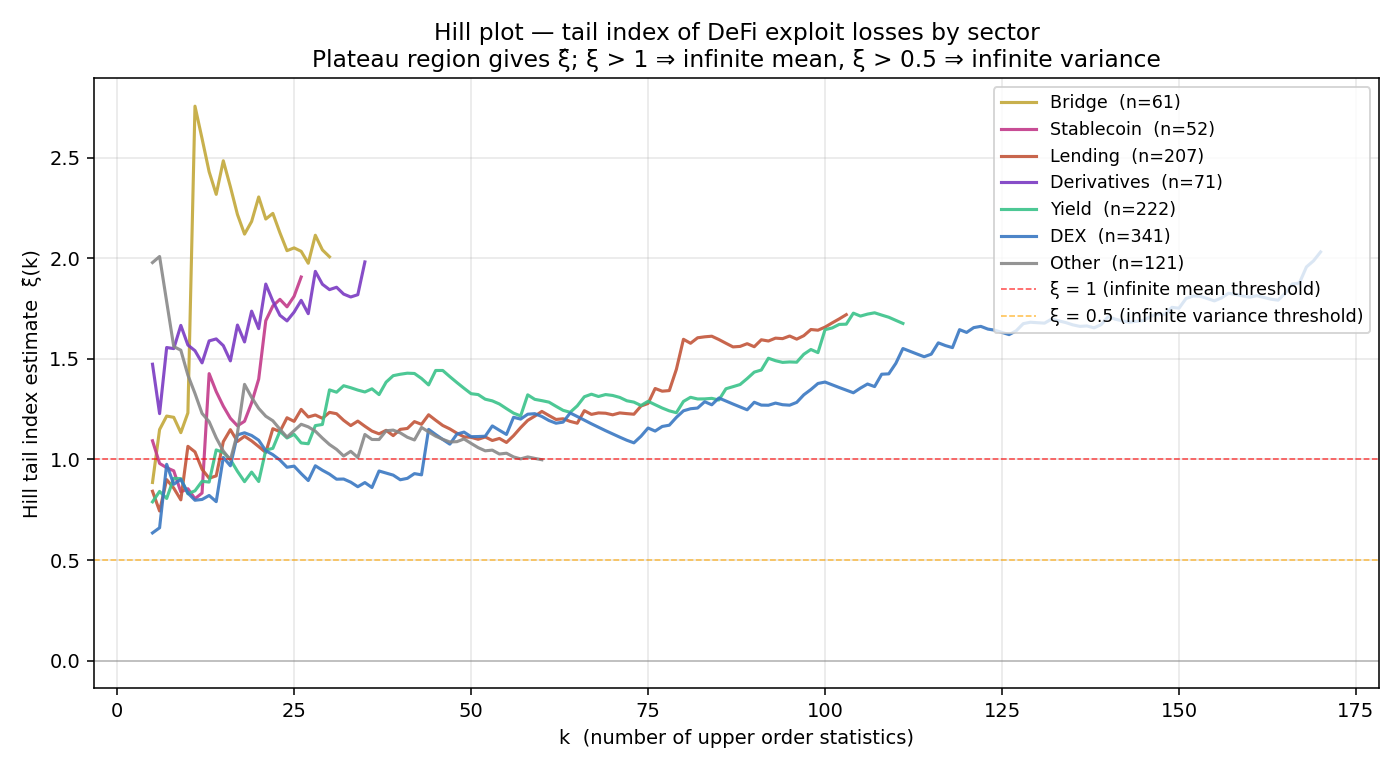
\includegraphics[width=0.86\linewidth]{r2_hill_plot.png}
\caption{Hill tail-index estimate $\hat\xi_H(k)$ per sector against the number
of upper order statistics $k$. A stable plateau in $k$ is the usable estimate.
Bridge sits above the infinite-mean line $\xi=1$ (red dashed); the remaining
sectors sit below it, between the infinite-variance line $\xi=0.5$ (orange
dashed) and $1$. The split reproduces the POT-GPD ordering by an independent
estimator.}
\label{fig:hill}
\end{figure}

\subsection{Step 3: quantifying uncertainty in $\hat\xi$}

Each $\hat\xi$ carries a $1{,}000$-replicate \emph{parametric bootstrap} $95\%$
CI. ``Parametric'' means I simulate fresh datasets \emph{from the fitted GPD},
refit each, and read the $2.5$/$97.5$ percentiles of the refit $\hat\xi$'s.
This propagates sampling uncertainty honestly, and it is what lets the paper say
the Bridge CI $[0.79,2.74]$ \emph{straddles} the infinite-mean boundary: the
point estimate exceeds $1$, but the data cannot rule out a finite mean.

\paragraph{The threshold-stability scan.}
The plateau-stability rule is easiest to see as a picture. Figure~\ref{fig:threshstab}
plots $\hat\xi(q)$ against the threshold quantile $q$ on a fine grid, with the
bootstrap CI and interquartile range shaded at every $q$. The rule fires where
the curve flattens into a plateau, and the picture shows why the guard floors
matter. In the Bridge panel the estimate is stable from $q=0.50$ to $q=0.85$ and
then collapses at $q=0.90$, where only ten exceedances remain and the GPD MLE
flips into Weibull-bounded territory. That collapse is small-sample noise, not
signal, and the $n_u\ge 20$ and $n_u/n\ge 10\%$ floors are exactly what exclude
it. Reading the plot is the honest way to confirm that each headline $\hat\xi$
comes from a genuine plateau and not from a lucky single threshold.

\begin{figure}[t]
\centering
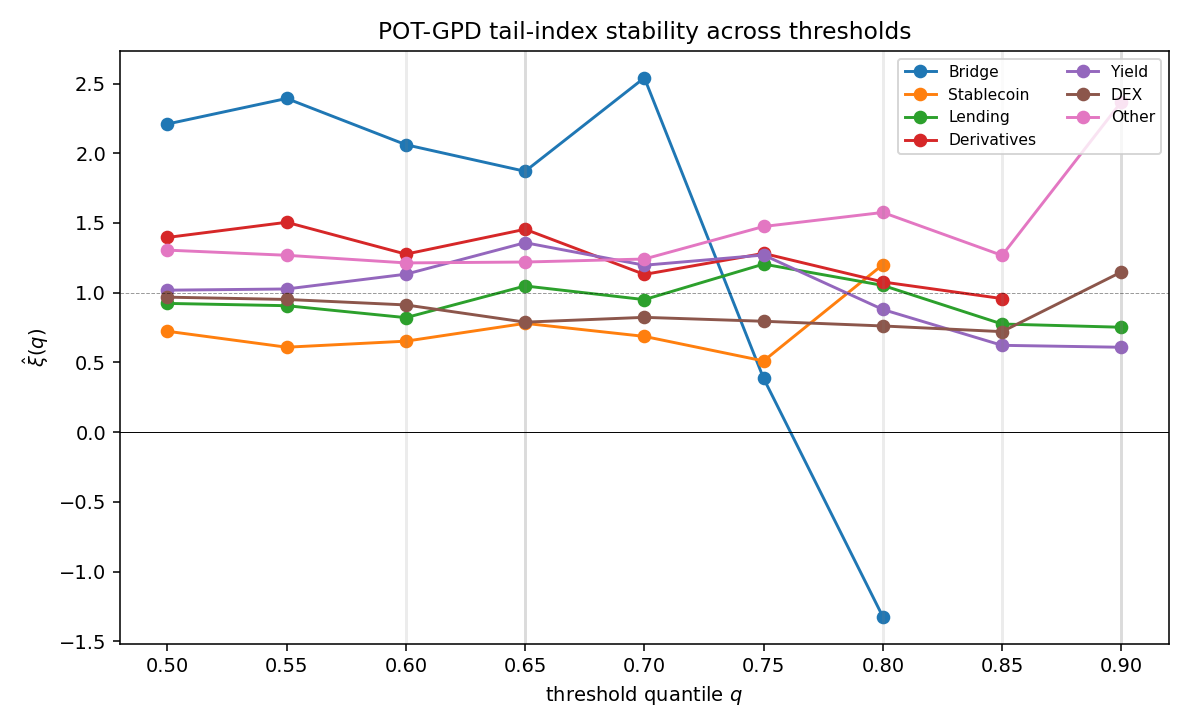
\includegraphics[width=\linewidth]{r5_xi_threshold_stability.png}
\caption{Per-sector parameter-stability scan: $\hat\xi(q)$ as a function of the
POT threshold quantile $q\in[0.50,0.90]$, step $0.05$. Number annotations are
the exceedance count $n_u$ at each $q$; red-ringed points flag $n_u<15$, where
the MLE asymptotics fail and the fit is unreliable. Shaded bands are the
$1{,}000$-replicate parametric bootstrap $95\%$ CI (light) and IQR (dark). A
flat region is a usable plateau; the Bridge collapse at $q=0.90$ ($n_u=10$) is
the small-sample instability the count floors are designed to exclude.}
\label{fig:threshstab}
\end{figure}

\subsection{Step 4: frequency by negative binomial}\label{sec:frequency}

For each sector I fit a count model to the \emph{monthly} event series,
$N_s\sim\NB(\mu_s,\alpha_s)$.

\paragraph{Why not Poisson?}
The natural first model is Poisson, whose defining property is
$\Var(N)=\E(N)$: events arrive independently at a constant rate. Real exploit
counts \emph{cluster} --- a new attack technique spawns copycats, a market crash
triggers correlated liquidations --- so the variance exceeds the mean. This is
\emph{over-dispersion}, and Poisson cannot represent it. The clustering is
visible directly in the rolling event intensity
(Figure~\ref{fig:rolling}): each sector's 90-day event rate rises and falls
in waves rather than fluctuating around a flat line, and the sector mix rotates
over time (the early rugpull wave in 2021, Bridge mega-events in 2022, a broad
lift in 2023). Two facts for the model follow from the same picture. The
waviness is the over-dispersion the negative binomial captures, and the
sector-mix rotation is the empirical warrant for fitting frequency
\emph{per sector} rather than pooling.

\begin{figure}[t]
\centering
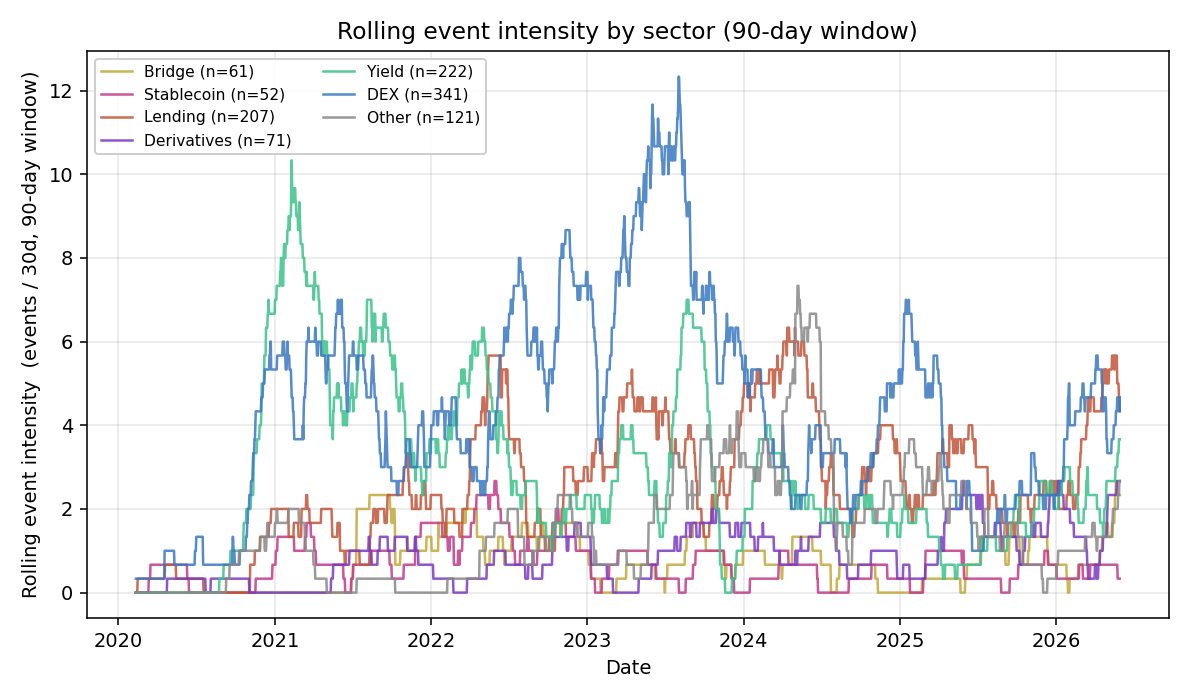
\includegraphics[width=0.92\linewidth]{r0c_rolling_intensity_sector.png}
\caption{Rolling 90-day event intensity by sector (events per 30-day
equivalent). Intensity moves in waves rather than around a constant rate, the
temporal clustering that over-disperses the monthly counts and rejects Poisson.
The relative sector composition also rotates over time, the descriptive warrant
for the per-sector treatment.}
\label{fig:rolling}
\end{figure}

\begin{assumption}[Event independence]\label{as:independence}
Conditional on the fitted frequency law, events arrive independently: an exploit
at one protocol does not raise the near-term hazard at another. The compound
model draws the annual count once and the severities independently, with no
self-excitation.
\end{assumption}

\noindent Assumption~\ref{as:independence} is the one the paper is most explicit
about violating. The wavy rolling intensity in Figure~\ref{fig:rolling} is exactly
the cross-protocol contagion a self-exciting (Hawkes) point process models, and
the negative binomial captures the resulting over-dispersion only in the
\emph{marginal} count, not the \emph{timing} dependence. The direction of the
error is known. Ignoring positive contagion understates the probability of a
cluster of large events in one year, so the reported $\VaR_{99.9}$ is, if
anything, a lower bound on the true tail. A joint Hawkes model is the natural
extension (Section~\ref{sec:assumptions}).

\paragraph{Fitting the whole window as one process.}
The same rolling-intensity picture that shows clustering also shows \emph{trend}:
the sector mix rotates and the overall level drifts across 2020--2026, so the
event rate is not constant over the window. I nonetheless fit one frequency law
(and one severity law) per sector on the full window.

\begin{assumption}[Stationarity]\label{as:stationarity}
The per-sector severity and frequency laws are constant over the 2020--2026
window, so a full-sample fit estimates the process that generates next year's
loss.
\end{assumption}

\noindent Assumption~\ref{as:stationarity} is visibly an idealization, in two
directions the same figure displays. Frequency fell from the early rugpull wave,
and severity moved toward larger, more concentrated targets. The paper's
out-of-sample backtest quantifies the cost, and the direction of the error runs
opposite to the independence one, so Section~\ref{sec:assumptions} takes the two
up together with the fix for each.

\paragraph{The negative binomial as a Gamma-mixed Poisson.}
Let the rate itself be random: $\Lambda\sim\text{Gamma}$, and
$N\mid\Lambda\sim\text{Poisson}(\Lambda)$. Marginalizing over $\Lambda$ gives a
negative binomial with
\begin{equation}\label{eq:nbvar}
\E(N)=\mu, \qquad \Var(N)=\mu+\alpha\mu^2,
\end{equation}
where $\alpha\ge 0$ is the \emph{dispersion}. At $\alpha=0$ the variance equals
the mean and I recover Poisson; $\alpha>0$ is over-dispersion, and larger
$\alpha$ means more clustering. Under-modeling dispersion would understate how
many events a bad year can hold, and hence understate $\VaR_{99.9}$ --- you
would report too little capital.

\paragraph{From monthly to annual: why the dispersion divides by 12.}
The compound~\eqref{eq:compound} needs an \emph{annual} count, which I take as
the sum of twelve iid monthly draws. The paper states
$\hat\alpha_{\text{annual}}=\hat\alpha_{\text{monthly}}/12$ in one clause; here
is the derivation. Using~\eqref{eq:nbvar}, twelve independent months give
\[
\E[N_{\text{yr}}]=12\mu, \qquad
\Var(N_{\text{yr}})=12(\mu+\alpha\mu^2)=12\mu+12\alpha\mu^2.
\]
Now require the annual count to be NB with mean $\mu'=12\mu$ and dispersion
$\alpha'$, so $\Var=\mu'+\alpha'\mu'^2=12\mu+\alpha'(144\mu^2)$. Matching the
two variance expressions,
\[
12\alpha\mu^2 = 144\,\alpha'\mu^2 \;\Longrightarrow\; \alpha'=\frac{\alpha}{12}.
\]
Intuition: aggregating independent periods averages out clustering, so a year
is proportionally \emph{less} over-dispersed than a single month.

\paragraph{The Poisson-versus-NB picture.}
Figure~\ref{fig:monthly} makes the over-dispersion visible in the count
distribution itself. The upper panel is the monthly event count over the sample;
the lower panel overlays the fitted Poisson and negative-binomial probability
mass functions on the observed histogram. The Poisson curve is too narrow: it
concentrates mass near its mean and assigns almost no probability to the busy
months of 30-plus events that actually occur. The negative binomial spreads mass
into exactly that right tail. Because the compound $\VaR_{99.9}$ is driven by
high-count years, the gap between the two curves in the right tail is the gap
between an adequate and an inadequate capital number.

\begin{figure}[t]
\centering
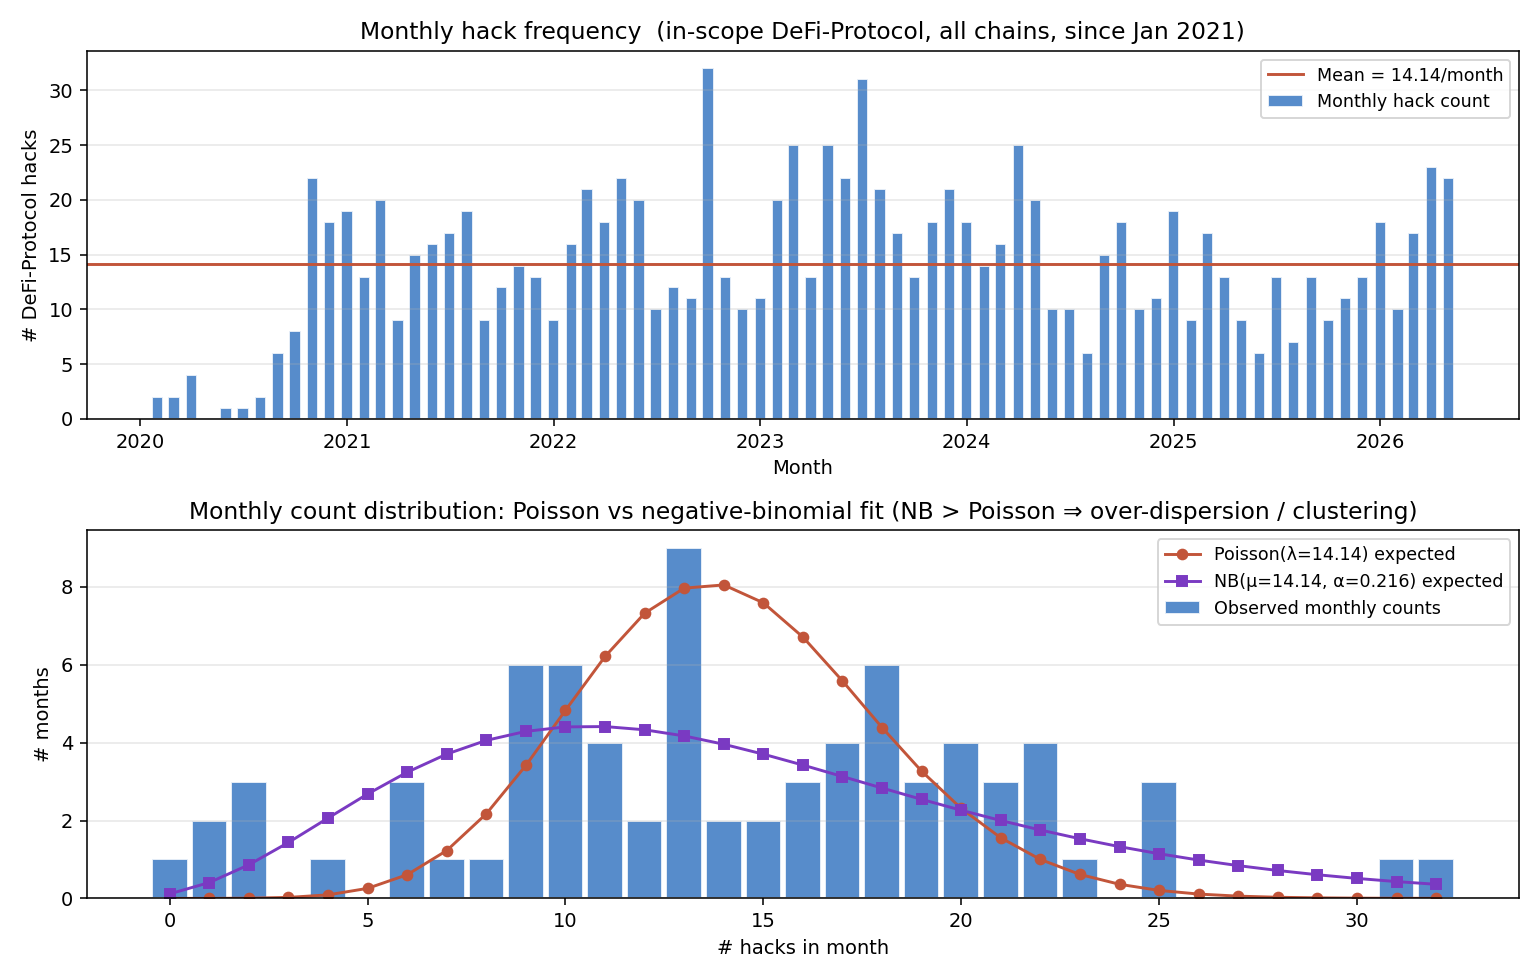
\includegraphics[width=0.92\linewidth]{r6_monthly_counts.png}
\caption{Monthly in-scope event counts (upper) and the cross-sector count
distribution with fitted Poisson and negative-binomial PMFs (lower). The
negative binomial ($\alpha\approx 0.2$) captures the right tail of busy months
that Poisson under-counts. Because the compound $\VaR_{99.9}$ is dominated by
high-count years, that right-tail mass is what a Poisson model would leave out of
the capital figure.}
\label{fig:monthly}
\end{figure}

\subsection{Step 5: compound aggregation by Monte Carlo}\label{sec:compound}

There is no closed form for a compound NB--GPD, so I simulate $2\times 10^5$
years per sector. Each simulated year: draw $N$ from the annual NB, draw $N$
severities from the empirical-body/GPD-tail mixture, and sum. From the
$200{,}000$ totals I read the mean $\E[S]$ (the \emph{pure premium}) and the
$0.999$ quantile $\VaR_{99.9}$ (the \emph{capital buffer}).

\paragraph{The exposure cap.}
Each simulated single-event loss is capped at the largest single-protocol
exposure in the sector, because one operational event cannot drain more than
the assets at risk in one protocol. This is not cosmetic. For the finite-mean
sectors it merely bounds the extreme quantile; for the $\xi>1$ sectors it is the
\emph{only} thing that makes $\VaR$ finite at all. The paper reports both the
capped figure and the uncapped $\VaR_{99.9}^{U}$, and the uncapped Bridge value
diverges to $286\times$ TVL --- a direct display of the infinite-mean pathology
(Section~\ref{sec:xi}).

\begin{assumption}[Exposure cap]\label{as:cap}
A single operational event cannot lose more than the assets at risk in one
protocol, so each simulated loss is truncated at the largest single-protocol
exposure in the sector.
\end{assumption}

\noindent Assumption~\ref{as:cap} is economically unimpeachable for a single
event, but it does real work in the results and the reader should see where. For
the finite-mean sectors it changes little. For Bridge and Derivatives ($\xi>1$)
it is load-bearing: without it there is no finite quantile at all, so the
reported Bridge and Derivatives capital figures are properties of the cap, not of
the fitted severity. The paper is explicit that these two rows are cap-determined
floors rather than estimates, which is why it declines to read them as capital
targets.

\paragraph{Expressing capital as a fraction of TVL.}
I report $\E[S]$ and $\VaR_{99.9}$ as a share of each sector's trailing-365-day
total value locked (TVL). The share is the meaningful unit --- it answers ``what
fraction of depositors' money'' --- and it respects the cap, since a protocol
cannot lose more than users supplied. One refinement matters and is worth making
explicit once. The TVL used as the denominator is the \emph{net} figure, the
idle assets actually sitting in the protocol, not the gross supplied total.
For a lending market, gross supplied TVL counts idle liquidity \emph{plus} funds
that have been borrowed out, and the borrowed portion has left the contract, so a
drain-the-pool operational event cannot take it. Net TVL strips the borrowed
leg back out and leaves the value genuinely exposed to an operational loss. Using
net TVL also removes the recursive double-counting that inflates gross figures,
where the same dollar is supplied, borrowed, and re-supplied and would otherwise
be counted more than once. The paper does not repeat the word ``net'' on every
mention of TVL, but every capital number (the severity cap, $\E[S]$, and
$\VaR_{99.9}$) is computed on this net basis. The one place gross supplied TVL is
used is selecting which ten venues enter the sample, so that a high-utilization
money market is not understated at the selection step. Two sectors lack a clean
supply-side TVL, so I substitute the closest exposure base: decentralized-stablecoin
circulating supply for Stablecoin, and residual TVL for Other. Both are
approximate and flagged as such.

\begin{assumption}[TVL as the exposure base]\label{as:tvlbase}
Trailing-365-day \emph{net} TVL (idle assets held in the protocol, gross supply
less funds borrowed out) is \emph{taken as} the exposure base for capital and the
weight for allocating a sector loss to a protocol, because it is the pool of
depositor funds an operational event can actually reach and it keeps the capital
ratio consistent with the exposure cap (Assumption~\ref{as:cap}). Where a clean
supply-side net TVL does not exist, the closest available exposure base
substitutes (decentralized-stablecoin circulating supply for Stablecoin, residual
TVL for Other).
\end{assumption}

\noindent Assumption~\ref{as:tvlbase} is deliberately hedged. Net TVL is the
\emph{appropriate} at-risk base, not a provably unique one, which is why the
statement says ``taken as'' rather than asserting correctness. It is clean for the
supply-side sectors (Lending, DEX, Yield) where net TVL is well defined, and
admittedly approximate for Stablecoin and Other, whose substitute bases are
flagged and kept out of the adequacy tests. It is also where value-at-risk can
depart from locked value: gross TVL can still be inflated by mercenary,
incentive-chasing deposits, and a larger venue may be better audited so that risk
per dollar falls with size, the same concern the per-sector homogeneity
assumption (Assumption~\ref{as:homogeneity}) carries.

\subsection{Why I fit per sector, not once}\label{sec:persector}

I fit severity and frequency \emph{once per sector} rather than on the pooled
data. The reason is the orthogonality of Section~\ref{sec:oprisk}: the dominant loss
mechanism differs by sector (Bridge is EF on pooled collateral; Lending and
Stablecoin are CPBP economic-design failures). A single pooled fit would blend
these distinct loss-generating processes and misestimate every tail. The cost is
sample size --- only $60$ Derivatives events --- but the heterogeneity it
preserves is exactly what drives the per-sector capital numbers.

% ===========================================================================
\section{Reading the tail index $\xi$}\label{sec:xi}
% ===========================================================================

Everything downstream --- whether the mean exists, whether $\VaR$ is finite,
how capital scales with venue size --- is governed by where $\xi$ sits. This
short section is the conceptual heart of the paper.

\subsection{The moment rule and two thresholds}

\begin{proposition}[Finiteness of GPD moments]
For a GPD with shape $\xi>0$, the moment $\E[X^k]$ is finite if and only if
$k<1/\xi$. In particular the mean is finite iff $\xi<1$, and the variance is
finite iff $\xi<1/2$.
\end{proposition}

So two thresholds matter:

\begin{center}
\begin{tabular}{lll}
\toprule
$\xi$ range & Tail behavior & Finite moments \\
\midrule
$0<\xi<\tfrac12$ & heavy, finite variance & mean and variance \\
$\tfrac12\le\xi<1$ & heavy, \emph{infinite} variance & mean only \\
$\xi=1$ & infinite-mean boundary & none (mean diverges) \\
$\xi>1$ & infinite mean & none \\
\bottomrule
\end{tabular}
\end{center}

\paragraph{Why $\xi>1$ is a crisis, not merely ``heavy.''}
If the mean is infinite, the sample average is not a consistent estimator of
anything: add more data and it keeps drifting up, dragged by the next record
event. A capital number built on such a severity \emph{diverges} --- there is
no stable $1$-in-$1000$ loss. This is precisely the instability that led the
Basel Committee to retire the internal-model Advanced Measurement Approach in
2017. The paper's Bridge ($\hat\xi=1.74$) and Derivatives ($\hat\xi=1.16$)
reproduce it: their point estimates cross the boundary, and only the exposure
cap gives them a finite $\VaR$. The paper is careful to add that both
confidence intervals straddle $1$, so the crossing is a point estimate, not an
inference.

\subsection{Subexponentiality and the single big loss}\label{sec:subexp}

\begin{definition}[Subexponential]
$F_X$ is subexponential if $\Prob(X_1+\dots+X_n>x)\sim\Prob(\max_i X_i>x)$ as
$x\to\infty$: a large sum is dominated by its largest term.
\end{definition}

All the paper's sectors are subexponential --- the diagnostics
(Section~\ref{sec:empirical}) confirm either a power-law or a lognormal tail, and both
are subexponential. This property is what makes ``a bad year is one bad event''
literally true, and it is what licenses the single-loss approximation for
per-protocol capital in Section~\ref{sec:allocation}.

\subsection{Tail index versus power-law exponent}

A GPD tail \emph{is} a power law: $\Prob(X>x)\sim x^{-1/\xi}$, so the CCDF
exponent is $1/\xi$. The paper also reports a Clauset power-law fit
$\hat\alpha_{\text{PL}}$, but Clauset's convention is the exponent of the
\emph{density}, $p(x)\sim x^{-\alpha}$, so the CCDF exponent there is
$\alpha-1$. Reconciling the two conventions,
\begin{equation}\label{eq:xialpha}
\xi \;\approx\; \frac{1}{\alpha_{\text{PL}}-1}.
\end{equation}
This is a useful order-of-magnitude cross-check between two independent fits:
Bridge's $\hat\alpha_{\text{PL}}=1.43$ implies
$\xi\approx 1/(1.43-1)=2.33$ against a fitted $1.87$, and DEX's $1.90$ implies
$1/(1.90-1)=1.11$ against $0.72$. The two fits agree on the heavy-versus-light
ordering, with the Hill-type $\hat\alpha_{\text{PL}}$ (evaluated at $u^*$)
running somewhat heavier than the GPD MLE.

% ===========================================================================
\section{Per-protocol allocation}\label{sec:allocation}
% ===========================================================================

The adequacy tests in Section~\ref{sec:responses} compare a \emph{specific venue's}
buffer or yield against \emph{its own} modeled capital. But no single protocol
records enough events for its own fit. Bridging that gap is a subtle and
important step.

\subsection{The credibility-theory framing}

When an individual unit has too little data for its own estimate, actuarial
\emph{credibility theory} (B\"uhlmann 1967; B\"uhlmann--Gisler 2005) prescribes
how much weight to place on that thin individual signal versus a broader
\emph{collective}. This is exactly my position. A single protocol records a
handful of events at most, far too few for its own tail fit, while its sector
pools hundreds. Credibility theory is the principled bridge between the two, and
it is worth spelling out because it is what licenses the whole per-protocol
allocation.

\paragraph{The credibility estimator.}
Let each protocol $p$ carry an unknown risk parameter $\Theta_p$, and let
$\mu(\Theta_p)=\E[X\mid\Theta_p]$ be its true, unobserved loss rate. The
credibility estimate of $\mu(\Theta_p)$ is a convex combination of the protocol's
own experience and the collective mean,
\begin{equation}\label{eq:cred}
\hat\mu_p \;=\; Z_p\,\bar X_p \;+\; (1-Z_p)\,\mu_0,
\end{equation}
where $\bar X_p$ is protocol $p$'s own average loss, $\mu_0$ the sector
(collective) mean, and $Z_p\in[0,1]$ the \emph{credibility factor}. Equation
\eqref{eq:cred} is the best linear approximation to the Bayesian posterior mean
$\E[\mu(\Theta_p)\mid\text{data}]$, which is why it is the standard actuarial
answer to ``trust the unit or trust the pool.'' At $Z_p=1$ I use the protocol's
own number; at $Z_p=0$ I hand it the sector's.

\paragraph{What sets the weight $Z$.}
In the B\"uhlmann--Straub model, where each unit carries an exposure (volume)
measure $w_p$, the credibility factor is
\begin{equation}\label{eq:Z}
Z_p \;=\; \frac{w_p}{w_p + k}, \qquad
k \;=\; \frac{\sigma^2}{\tau^2}
   \;=\; \frac{\E[\Var(X\mid\Theta)]}{\Var(\E[X\mid\Theta])}.
\end{equation}
The constant $k$ is the ratio of the \emph{expected process variance} $\sigma^2$
(the noise \emph{within} a unit's own history) to the \emph{variance of the
hypothetical means} $\tau^2$ (the genuine heterogeneity \emph{between} units).
The entire content of credibility theory sits in this one fraction. The weight
$Z_p\to1$, so I trust the unit, when its exposure $w_p$ is large or when units
are truly different ($\tau^2$ large, hence $k$ small). The weight $Z_p\to0$, so
I trust the pool, when the unit is data-poor or when units are essentially alike
($\tau^2$ small, hence $k$ large). Credibility rises with own data and with real
between-unit heterogeneity, and falls when either is missing.

\paragraph{Where this paper sits: near-total shrinkage.}
Two features of DeFi drive me to the $Z_p\to0$ corner. First, per-protocol event
counts are tiny, so $\bar X_p$ is almost pure noise and carries little weight in
its own right. Second, I do not attempt to estimate the between-protocol
heterogeneity $\tau^2$ at all, which is the same as treating $\tau^2\to0$, so
$k\to\infty$ and $Z_p\to0$ regardless of exposure. Both send the weight to zero,
and \eqref{eq:cred} collapses to $\hat\mu_p=\mu_0$: each protocol inherits the
\emph{sector} estimate outright. The natural volume measure $w_p$ in
\eqref{eq:Z} is net TVL, so ``inherit the sector estimate'' means ``inherit it
per unit of TVL,'' which is exactly the TVL-share thinning of the next
subsection, $\lambda_p=(\TVL_p/\TVL_s)\lambda_s$ with the shared severity. The
per-protocol allocation is thus a credibility estimate pinned at zero own-credibility.

\begin{assumption}[Per-sector homogeneity]\label{as:homogeneity}
All protocols in a sector share one severity law and one per-TVL event rate. A
sector event lands on protocol $p$ with probability proportional to its TVL
share $\TVL_p/\TVL_s$, and conditional on being struck, $p$'s loss is drawn from
the same $F_X$ (capped at its own exposure).
\end{assumption}

\noindent Assumption~\ref{as:homogeneity} is the price of thin per-protocol data,
and it is the one a referee will press hardest. It says risk-per-dollar is
constant within a sector, which a larger or more complex venue may violate by
carrying more risk per dollar of TVL. The paper flags this as the
\emph{homogeneity} limitation and names the fix: a size covariate or a
hierarchical (random-effects) severity model that lets each protocol's tail
depart from the sector collective as its own data accumulate. Absent that data
today, the TVL-share allocation is the disciplined default, and the credibility
framing is precisely the statement that it is a shrinkage estimate, not a claim
of true equality.

\subsection{Thinning the sector process to a protocol}

Model the sector's event stream and \emph{thin} it to a protocol by TVL share.
Let $\TVL_p$ be protocol $p$'s TVL and $\TVL_s=\sum_{p\in s}\TVL_p$ the sector
total. A sector event strikes protocol $p$ with probability $\TVL_p/\TVL_s$, so
$p$ inherits a thinned rate
\[
\lambda_p \;=\; \frac{\TVL_p}{\TVL_s}\,\lambda_s,
\]
the same per-event severity, capped at its own exposure.

\paragraph{The mean thins linearly.}
Because expectation is linear, the pure premium allocates cleanly by TVL share:
\[
\E[S]_p \;=\; \frac{\TVL_p}{\TVL_s}\,\E[S]_s.
\]
So if I only cared about the average, per-protocol numbers would be a trivial
rescaling. I care about the tail, and the tail does \emph{not} thin linearly.

\subsection{Why the tail scales as $\TVL_p^{\xi}$}\label{sec:tvlscaling}

For subexponential severity, the \emph{single-loss approximation}
(B\"ocker--Kl\"uppelberg 2005; Embrechts et al.\ 1997) says a high-quantile
aggregate $\VaR$ is essentially the matching severity quantile:
\begin{equation}\label{eq:sla}
\VaR_{0.999}(S_p) \;\approx\; F_X^{-1}\!\Bigl(1-\tfrac{0.001}{\lambda_p}\Bigr).
\end{equation}
Now use the GPD quantile, which for a small tail probability $pr$ behaves like
$F_X^{-1}(1-pr)\propto pr^{-\xi}$. Substituting $pr=0.001/\lambda_p\propto
1/\TVL_p$,
\[
\VaR_{0.999}(S_p) \;\propto\; \Bigl(\tfrac{1}{\TVL_p}\Bigr)^{-\xi}
\;=\; \TVL_p^{\,\xi}.
\]
Therefore the \emph{$\VaR$-to-TVL ratio} scales as $\TVL_p^{\xi-1}$. With
$\xi<1$ the exponent is negative, so \textbf{the smaller the venue, the larger
its capital as a share of its own TVL}. Intuitively, a small venue is struck
rarely, but when it is struck the loss is drawn from the same heavy severity
law, so relative to its size a bad year is proportionally more devastating.

\begin{remark}[Why I re-simulate rather than rescale]
Equation~\eqref{eq:sla} is why I cannot simply scale the sector $\VaR$-ratio
down to each protocol --- that would understate the small venues. I instead
re-simulate $\VaR_{99.9}$ per protocol. This is exactly why, in the yield table
(Section~\ref{sec:responses}), the per-protocol $\VaR_{99.9}$ premia
($5{,}998$--$9{,}666$~bps) dwarf the sector ratio ($\sim 1{,}800$~bps).
\end{remark}

% ===========================================================================
\section{Reading the empirical fits}\label{sec:empirical}
% ===========================================================================

A guided tour of the paper's tables and figures, and what each licenses.

\paragraph{Severity fits (Table 4).}
The per-sector $\hat\xi$, read against the two thresholds of Section~\ref{sec:xi} and
the Moscadelli (2004) banking band $[0.85,1.39]$:

\begin{center}
\begin{tabular}{llL{6.9cm}}
\toprule
Sector & $\hat\xi$ & Reading \\
\midrule
Bridge & 1.87 & past infinite-mean boundary; CI $[0.58,3.18]$ straddles it; cap-dependent \\
Other & 1.58 & past boundary; residual bucket, thin fit; cap-dependent \\
Derivatives & 1.45 & past boundary; only $71$ events; unstable \\
Lending & 0.75 & heavy, finite mean; sensitive to Vires Finance (single event) \\
DEX & 0.72 & heavy, finite mean; carried by many events \\
Stablecoin & 0.65 & moderately heavy, finite mean \\
Yield & 0.61 & moderately heavy, finite mean \\
\bottomrule
\end{tabular}
\end{center}

\noindent The understated headline: \emph{the four finite-mean DeFi sectors are
no heavier-tailed than banks}. The drama is not exotic tails but ordinary-heavy
tails combined with no capital.

\paragraph{Cross-tabulation (Table 3) and severity figures.}
The sector$\times$Basel table shows Bridge$\times$EF alone is $33\%$ of all
losses, and confirms that mechanisms differ by sector --- the empirical warrant
for per-sector fitting (Section~\ref{sec:persector}). The two severity figures
make the same point visually. The violin plot (Figure~\ref{fig:violin}) shows
that the per-sector loss distributions do not overlay: they differ in both
location and shape, so a single pooled severity would blend genuinely different
distributions. Bridge carries the highest median event loss, from the large
pooled collateral cross-chain bridges hold. The log-log CCDF
(Figure~\ref{fig:ccdf}) shows approximately straight tails, and a straight line
on log-log axes \emph{is} a power law, with slope the tail exponent. The two
plots are complementary: the violin reads the body and the CCDF reads the tail,
and both refuse to collapse the sectors onto one curve.

\begin{figure}[t]
\centering
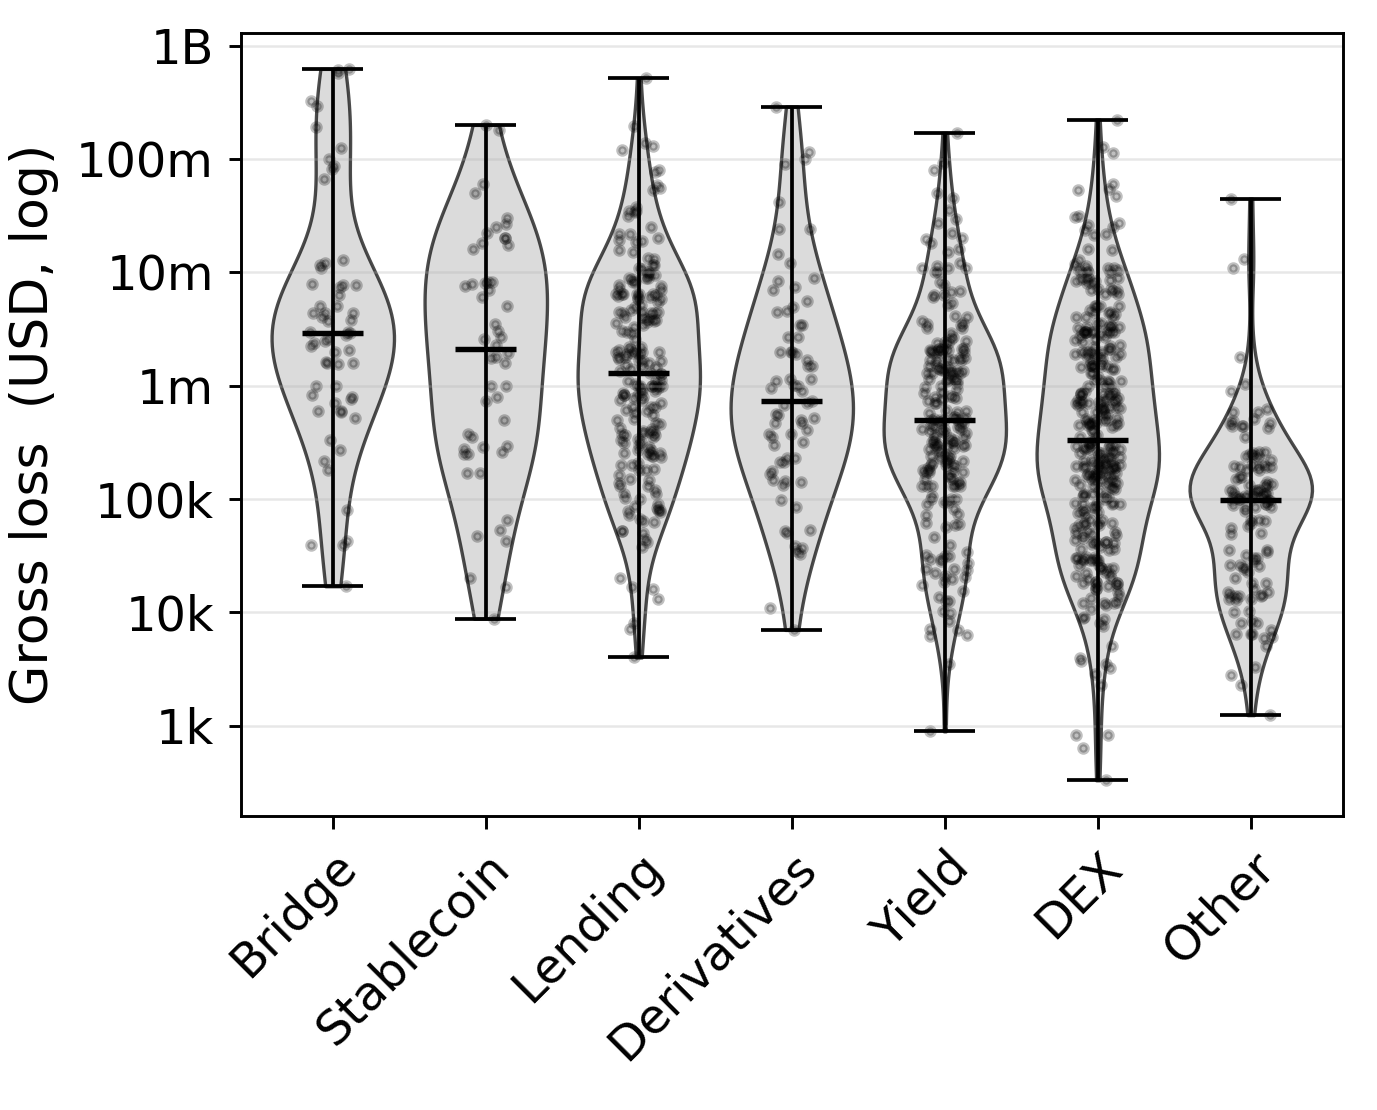
\includegraphics[width=0.55\linewidth]{r0b_violin_bw.png}
\caption{Per-sector loss distribution ($n=1{,}075$; violin = density, bar =
median), sectors by descending median. The violin reads the body
of the severity distribution and shows the sectors do not overlay in location or
shape, so a single pooled severity would blend genuinely different distributions.
Bridge carries the highest median event loss, from the large pooled collateral
cross-chain bridges hold.}
\label{fig:violin}
\end{figure}

\begin{figure}[t]
\centering
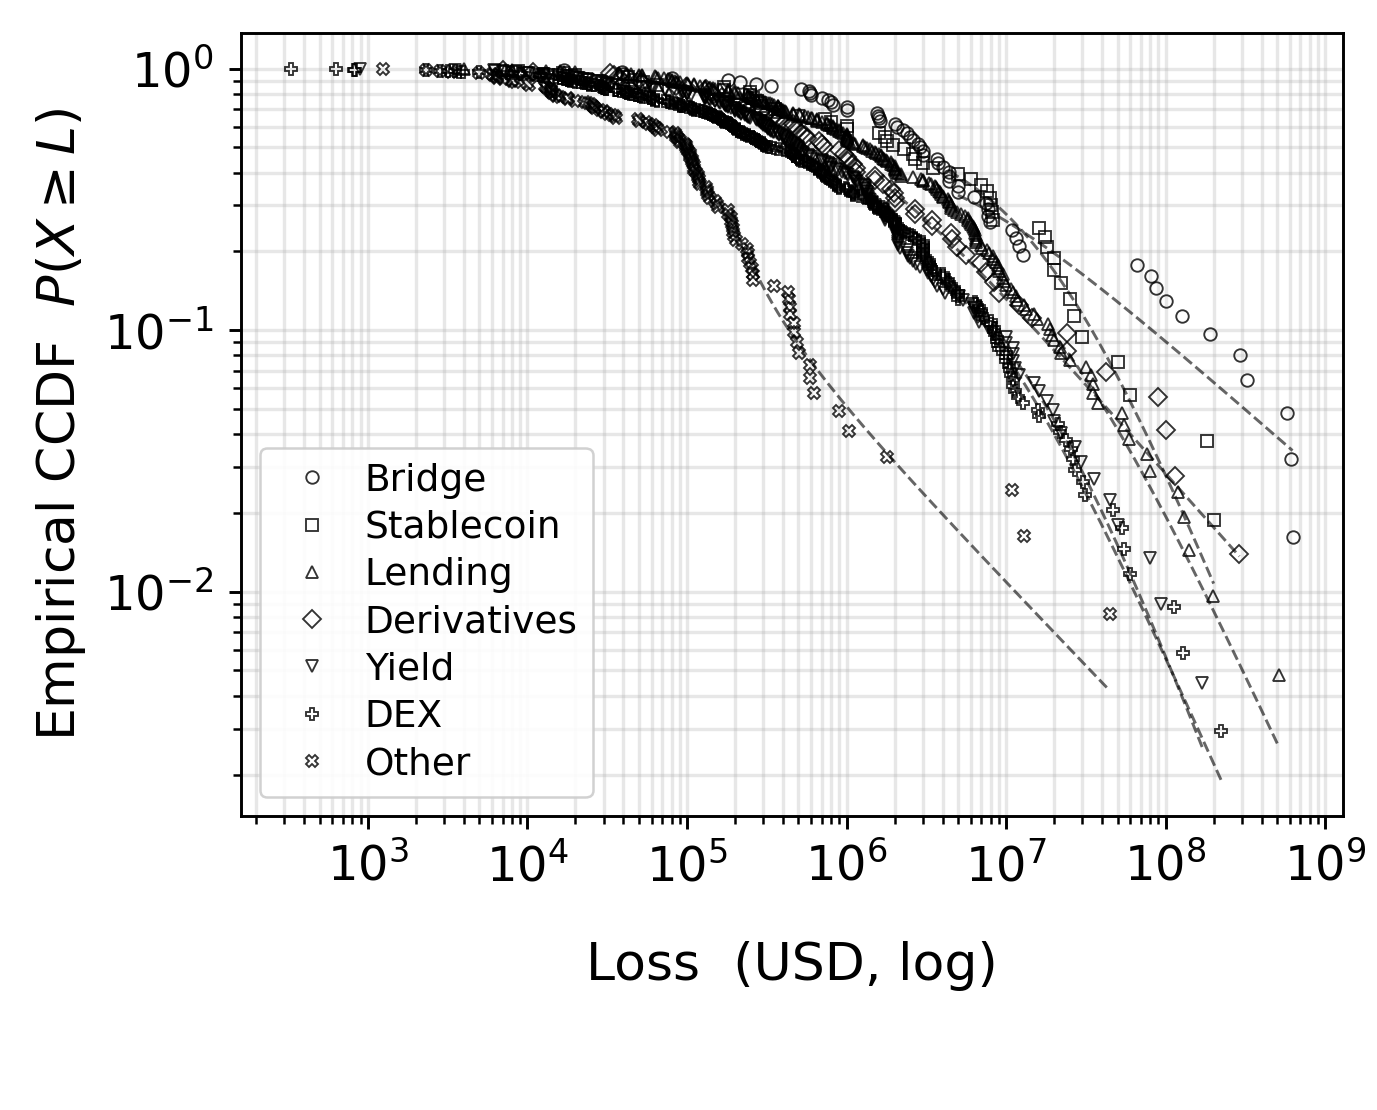
\includegraphics[width=0.55\linewidth]{r3_ccdf_bw.png}
\caption{Log-log complementary CDF $\Pr(X\ge L)$ per sector ($n=1{,}075$) with
the Clauset power-law tail (dashed) overlaid. The CCDF reads the tail and shows
approximately straight-line behavior over three decades, and a straight line on
log-log axes \emph{is} a power law with slope the tail exponent. Together with
the violin (Figure~\ref{fig:violin}) it is the descriptive warrant for a
per-sector, heavy-tailed severity model.}
\label{fig:ccdf}
\end{figure}

\paragraph{Frequency fits (Table 5).}
Annual rates run from $8.3$/yr (Stablecoin) to $54.2$/yr (DEX). The
likelihood-ratio column rejects Poisson in favor of NB in every sector but
the two smallest (Stablecoin, $p=0.59$; Derivatives, $p=0.05$), and a
cross-sector Cameron--Trivedi test gives an overwhelming dispersion index
$D=3.27$ ($z\approx14$).

\paragraph{Per-sector capital (Table 6).}
The yardstick itself, in \% of TVL, reported both capped and uncapped
($\VaR_{99.9}^{U}$). Lending $18.0\%$, Stablecoin $16.1\%$, Yield $15.3\%$,
DEX $14.1\%$ --- all far above the operational-risk capital banks hold. Bridge
$32.5\%$, Other $27.5\%$, and Derivatives $22.8\%$ are larger but
\emph{cap-determined}: uncapped, Bridge diverges to $673\times$ TVL.

\paragraph{Goodness of fit, and what each test assures.}
A capital number is only as trustworthy as the fit beneath it, so the paper runs
four separate goodness-of-fit checks, each closing a different failure mode.
\emph{(i) The QQ panel} (Figure~\ref{fig:qqpanel}) plots empirical excesses
against the fitted-GPD quantiles per sector. A near-straight $45^\circ$ line
means the fitted tail matches the data at every quantile, not just on average,
which is the check that matters for a $99.9\%$ number. The panel is essentially
straight in every sector, with a slight upper-tail over-shoot in Lending (Vires
Finance, Euler~V1) and Bridge (Ronin, Poly) where the data are very slightly
\emph{heavier} than the fit, so the reported figures there are, if anything,
mildly conservative. \emph{(ii) Kolmogorov--Smirnov distances} $\le 0.19$ (within
the $5\%$ critical band) give a formal, single-number version of the same
statement: the fitted and empirical tails are not statistically distinguishable.
\emph{(iii) The Vuong power-law-versus-lognormal test} is near-tied for the
lighter-tailed core sectors and favors the power law for the heavy-tailed ones
(Bridge, DEX, Other; $\text{LR}_{\text{LN}}>0$). This does not unsettle the
capital story: power-law and lognormal are both subexponential
(Section~\ref{sec:subexp}), so the $99.9\%$ figure is identical either way, and
where the test does discriminate it points to the heavier power-law tail,
consistent with the infinite-mean point estimates in those sectors. \emph{(iv) The frequency side} is checked by the
per-sector likelihood-ratio test (rejects Poisson at $p\le0.02$ in every
sector but the two smallest, Stablecoin and Derivatives) and the cross-sector
Cameron--Trivedi dispersion index $D=3.27$ ($z\approx14$), which together
certify that the negative binomial, not Poisson, is the right count law.

\begin{figure}[t]
\centering
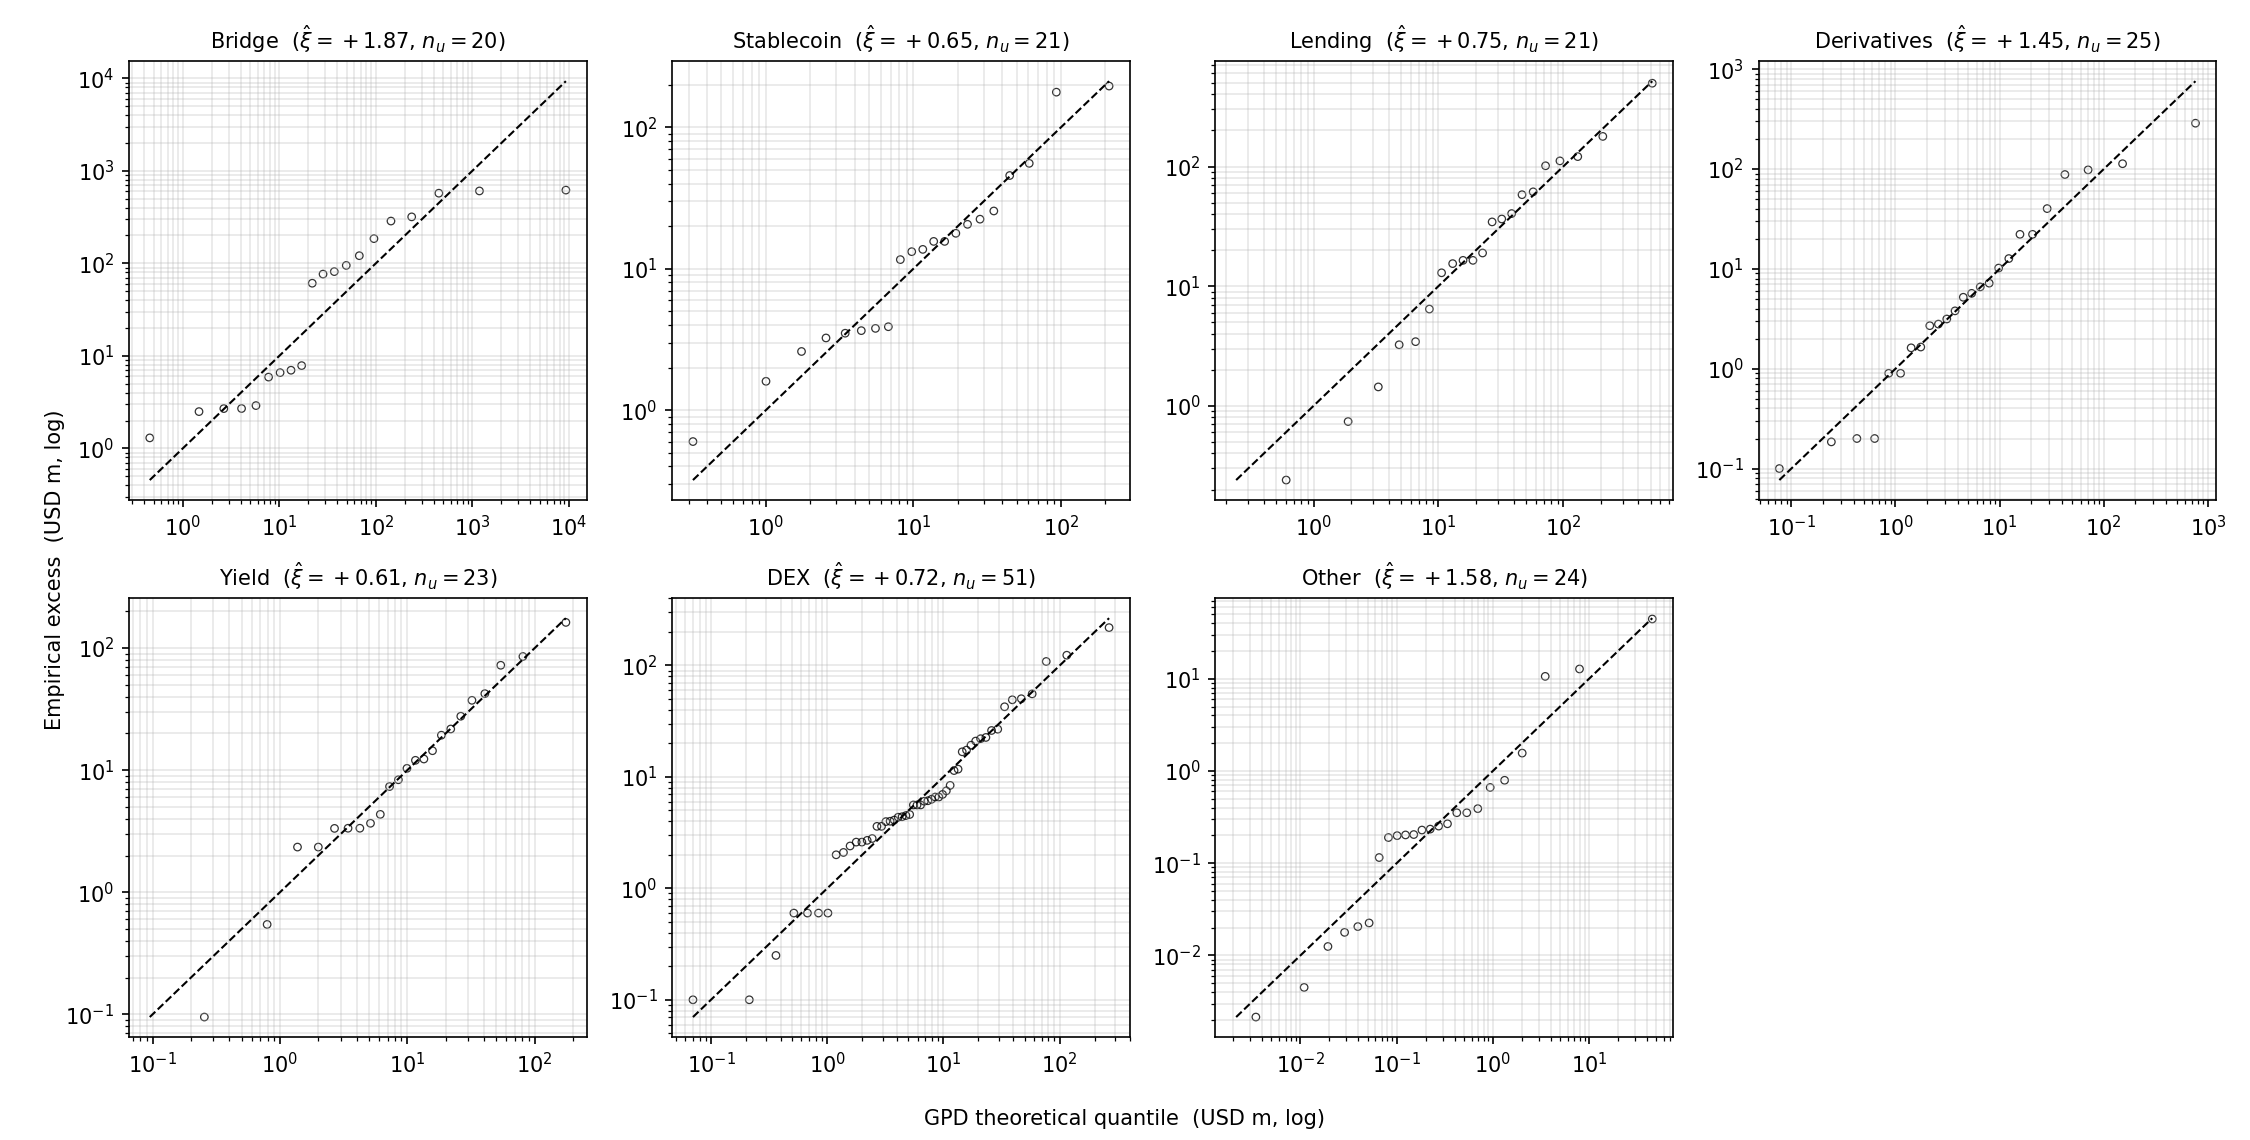
\includegraphics[width=\linewidth]{r4_gpd_qq_all_sectors.png}
\caption{Per-sector POT-GPD QQ diagnostic. Each panel plots empirical excesses
$X-u^*\mid X>u^*$ against the fitted-GPD theoretical quantiles at the headline
threshold, with the red dashed line $y=x$. A straight line certifies the tail
fit at every quantile, the property a $99.9\%$ capital number depends on. The
moderate-tail sectors align across the full tail; Lending and Bridge show a
slight upper-tail over-shoot (data heavier than the fit), so their figures are
mildly conservative.}
\label{fig:qqpanel}
\end{figure}

\paragraph{Robustness, and what each check rules out.}
Three sensitivity checks bound the ways the headline could be an artifact.
\emph{(i) Drop the largest events} asks whether the tail hangs on a single
event. Tail-index estimates are known to be sensitive to a handful of extremes
(Embrechts--Kl{\"u}ppelberg--Mikosch 1997) and the DeFi fits are no exception:
dropping the single largest event moves $\hat\xi$ by $0.2$--$0.4$ in most
sectors, most sharply in Lending ($\hat\xi=0.75\to0.35$ without Vires Finance).
Bridge and DEX are essentially unchanged --- their tails are carried by many
events rather than one. Under any drop-top rule up to $0.5\%$, however, every
sector retains its below/above infinite-mean characteristic (Lending,
Stablecoin, Yield, DEX below $\hat\xi=1$; Bridge, Derivatives, Other above),
so the qualitative conclusion is unchanged even as point estimates move.
\emph{(ii) Cap sensitivity} asks how much of the capital number is the exposure
cap (Assumption~\ref{as:cap}) rather than the severity fit. Uncapped, Lending
rises $18\%\to22\%$, DEX $14\%\to46\%$, Yield $15\%\to30\%$, and Bridge
diverges, so the reported figures are cap-bounded floors and should be read as
such. \emph{(iii) Confidence level} asks whether the conclusion depends on the
stringent $99.9\%$ benchmark. Lowering it to $99.5\%$ and $99\%$ cuts Lending
capital $18\%\to7\%\to5\%$ and lifts buffered-venue coverage $5\%\to18\%\to32\%$,
but even at $99\%$ the buffer covers only about a third of a requirement that
is still an order of magnitude above bank operational-risk capital. The
finding is therefore not an artifact of the confidence level. A fourth check,
the out-of-sample backtest, is discussed under stationarity in
Section~\ref{sec:assumptions}.

% ===========================================================================
\section{The two responses and the substitution test}\label{sec:responses}
% ===========================================================================

Now I use the yardstick. Every comparison here is an \emph{adequacy} test:
observed margin against modeled requirement.

\subsection{Response 1: protocol capital buffers (Table 7)}

Take the ten largest Lending venues by gross supplied TVL (June~2026). Four
disclose an operational-risk reserve (Aave~V3, SparkLend, Compound~V3, Venus);
six hold nothing. Apply the per-protocol allocation of Section~\ref{sec:allocation}
to get each venue's $\E[S]$ and $\VaR_{99.9}$.

\paragraph{The two-layered finding.}
Against the pure premium $\E[S]$, all four buffers are ample ---
coverage $159\%$--$599\%$. Against the tail $\VaR_{99.9}$, all four
\emph{collapse} to $2\%$--$9\%$ coverage, a $\sim 95\%$ average shortfall. A
buffer sized to the average is nowhere near sized to the tail --- precisely
because the tail is heavy. Confusing $\E[S]$ with tail capital is the exact
error the paper exists to expose.

\subsection{Response 2: depositor yield premia (Table 8)}

Where the protocol holds no buffer, the residual falls on the depositor, who
should be paid a risk premium. I measure it as
\[
\text{risk premium}
\;=\; \underbrace{\text{30-day TVL-weighted stablecoin supply APY}}_{\text{what the depositor actually earns}}
\;-\; \underbrace{3.70\%}_{\text{3-month T-bill (FRED DTB3)}}.
\]

\paragraph{The finding.}
Across the unbuffered venues the premium averages $+54$~bps --- but the pure
premium alone is $64$~bps, and the tail-risk premium (per-protocol
$\VaR_{99.9}$) is $34$--$81\%$ of TVL, thousands of bps. So the premium does
not even cover the average, let alone the tail. The cross-section is wide,
from $+257$~bps (Fluid) to $-79$~bps (Kamino), and three venues pay
\emph{below} the risk-free rate while exposing depositors to an uncapped tail.

\paragraph{An honesty flag.}
The spread is a \emph{proxy}, not an identified price. The supply yield also
reflects utilization, rate governance, protocol-idiosyncratic risk, and
incentives. This is a reduced-form measurement; a controlled panel regression
is the natural extension.

\begin{assumption}[Yield spread as the risk premium]\label{as:yieldproxy}
The excess of the TVL-weighted stablecoin supply APY over the 3-month T-bill is
the depositor's compensation for operational risk. The risk-free benchmark is
the T-bill at $3.70\%$.
\end{assumption}

\noindent Assumption~\ref{as:yieldproxy} is deliberately the weakest link on the
depositor side, and the paper says so. The spread is not identified: it also
moves with utilization and incentives, so it over- or under-states the
operational-risk premium by an unknown amount. Two features keep the conclusion
robust despite this. The gap being measured is an order of magnitude (tens of
bps against a $\sim1{,}800$-bps tail), far larger than any plausible mislabeling
of the spread, and the benchmark choice is checked: under SOFR, sUSDS, or the
Coinbase USD rate the excess yield stays at or below zero. A panel regression
that controls for utilization and incentives is the identified-price extension.

\subsection{Do the two margins substitute? The Mann--Whitney test}\label{sec:mwtest}

The efficient-market prediction (Section~\ref{sec:setup}) is that buffered venues,
having pre-funded the tail, should pay \emph{lower} yield. I test it.

\paragraph{Why a rank test.}
With only ten venues and non-normal premia with outliers, a $t$-test is
inappropriate. I use a one-sided \emph{Mann--Whitney $U$ test} (Wilcoxon
rank-sum), which compares the \emph{ranks} of the two groups' premia and makes
no normality assumption. The one-sided alternative encodes the directional
economic hypothesis: buffered $<$ unbuffered.

\paragraph{The result, and its two halves.}
The buffered median premium is $-86$~bps against $+39$~bps unbuffered --- a
$125$~bps gap --- with one-sided $p=0.01$. The \emph{direction} is real and
significant. But the whole premium cross-section spans just $418$~bps, while the
tail demands $\sim 18\%$ of TVL. So:
\begin{quote}
The market prices operational risk \emph{in the right direction} but an order
of magnitude too small. Both margins together leave the tail overwhelmingly
unfunded.
\end{quote}
This one sentence is the paper's synthesis --- the substitution result
(direction) and the adequacy result (magnitude) held together.

\subsection{From result to policy}

\paragraph{Who bears the shortfall.}
The premium I measure is the posted supply APY --- the rate a retail depositor
sees and takes. A professional can assess the tail, negotiate bilateral terms,
and size or exit; a retail depositor sees only the posted rate and, lacking
standardized disclosure, cannot judge whether the yield compensates the risk
(Cornelli et al.\ 2025 on search-for-yield). So the unpriced tail lands
disproportionately on the least-equipped party.

\paragraph{Why disclosure, not capital mandates.}
Because a decentralized protocol may have no responsible legal entity, a
bank-style capital mandate is hard to impose. What market discipline requires is
\emph{information}, and the LDA supplies its content. The paper recommends a
Pillar-3 analogue --- standardized loss-and-yield disclosure, buffer-and-tail
disclosure, periodic recalibration --- and notes the duty can attach to whoever
\emph{fronts} access (front-ends, wallets, aggregators, custodial ``earn''
products), the identifiable points where a retail depositor actually enters.

\paragraph{A pointer on limitations.}
The obvious referee objections to the two responses --- that the buffer--yield
association is descriptive rather than causal, that the yield spread is a proxy,
that the sample is only ten venues --- are limitations of the assumptions behind
the tests. Section~\ref{sec:assumptions} takes them up together with every other
modeling assumption, stating for each the limitation it implies and the fix.

% ===========================================================================
\section{Assumptions, the limitations they imply, and how to fix them}\label{sec:assumptions}
% ===========================================================================

Every headline number rests on a chain of modeling assumptions, each stated at
its natural point above. This section collects all nine in one place and, for
each, names the limitation it implies and the extension that would fix it. It
also adds the one limitation that is not a modeling assumption but a property of
the ten-venue sample. There are no subsections by design. The aim is a single
readable map of where the next paper on this dataset should go.

\emph{The assumptions and their fixes at a glance.}
Table~\ref{tab:assumptions} lists the nine assumptions, each with the direction
of the error it induces and the extension that would weaken it. Read the
``direction of error'' column as the answer to ``if this assumption is wrong,
which way is the reported capital number biased?'' The recurring pattern is worth
naming: almost every assumption biases the capital figure \emph{downward} or
leaves the tail untouched. Incomplete data lightens only the body, gross losses
overstate nothing, ignored contagion understates cluster years, and the earlier
window understates the later tail. The reported inadequacy is therefore
conservative. Relaxing the assumptions would, on the balance of the signed
errors, widen the gap between the risk and its funding rather than close it.

\begin{table}[t]
\centering
\footnotesize
\begin{tabular}{@{}L{2.5cm} L{4.0cm} L{2.6cm} L{4.0cm}@{}}
\toprule
Assumption & What it buys & Direction of error & Extension that weakens it \\
\midrule
Gross loss and reporting completeness (A\ref{as:gross}) &
Uses reported losses directly; no recovery model &
Conservative: nets nothing, lightens only the body &
Recovery-adjusted (net) severity; censoring model for small losses \\[2pt]
Compound structure (A\ref{as:compound}) &
Classical collective-risk form; tail of $S$ from $F_X$ alone &
Depends on the two below &
Joint severity--frequency and dependence modeling \\[2pt]
GPD tail (A\ref{as:tail}) &
Parametric tail, non-parametric body; one shape parameter $\xi$ &
Small ($u$ finite); tested by QQ, KS, mean-excess &
Higher threshold; second-order (penultimate) tail correction \\[2pt]
Event independence (A\ref{as:independence}) &
Draw $N$ once, severities iid; no timing model &
Understates cluster years, so $\VaR$ is a lower bound &
Self-exciting (Hawkes) point process on the same data \\[2pt]
Exposure cap (A\ref{as:cap}) &
Finite $\VaR$ even for $\xi>1$ sectors &
Load-bearing for Bridge, Derivatives; those rows are floors &
Per-protocol exposure paths; contagion-aware cap \\[2pt]
Net TVL as exposure base (A\ref{as:tvlbase}) &
Net (idle) TVL: capital as a share of at-risk depositor funds; respects the cap &
Approximate for Stablecoin and Other (flagged, not used) &
Supply-side net-exposure series per protocol \\[2pt]
Per-sector homogeneity (A\ref{as:homogeneity}) &
Per-protocol capital from thin data via TVL share &
Understates large/complex venues if risk-per-dollar rises with size &
Size covariate or hierarchical (random-effects) severity \\[2pt]
Yield spread as premium (A\ref{as:yieldproxy}) &
An observable depositor-side compensation measure &
Not identified; robust only because the gap is an order of magnitude &
Panel regression controlling for utilization and incentives \\[2pt]
Stationarity (A\ref{as:stationarity}) &
One full-sample fit per sector &
Earlier window understates the later tail (backtest) &
Regime-split fit; non-stationary background rate \\
\bottomrule
\end{tabular}
\caption{The nine modeling assumptions, what each buys, the direction in which
it biases the reported capital figure, and the extension that would relax it.
The recurring feature is that the signed errors point the same way: relaxing the
assumptions would, on balance, widen the risk-versus-funding gap the paper
reports, not close it.}
\label{tab:assumptions}
\end{table}

\emph{Stationarity is the limitation the backtest quantifies.} The frequency and
severity laws are fit on the full 2020--2026 window as if stationary
(Assumption~\ref{as:stationarity}), yet the rolling intensity of
Figure~\ref{fig:rolling} shows the process drifting. The out-of-sample backtest
puts a number on the cost. Refitting Bridge on the 2020--2023 sub-sample
($n=37$) yields a degenerate estimate --- the plateau selector falls back
because $n_u=11<20$ and the fitted $\hat\xi$ is not defensible --- while the
full 2020--2026 sample gives $\hat\xi=1.87$, driven by the Kelp bridge
exploit ($\$292$~m, 2026) that arrived only in the hold-out. Similarly large
2024--2026 events landed in other sectors: Cetus ($\$223$~m, DEX) and Drift
Trade ($\$285$~m, Derivatives). The lesson is not a specific drift number but
the structural one: for the heavy-tail sectors the 2020--2023 sample is
simply too small to fit a tail at all, and the full-sample figure is the
appropriate forward-looking estimator with the caveat that a single new
mega-event materially moves it. The Kupiec coverage $p$-values are
uninformative at a three-year hold-out, so reading the test as ``the model is
validated'' would over-claim. A regime-split fit or a non-stationary
background rate is the fix.

\emph{One limitation is not a modeling assumption: confounding in the
substitution test.} The buffer--yield association (Section~\ref{sec:mwtest}) is
descriptive, not causal. The buffered venues are also the largest and oldest, so
brand and perceived safety may drive the lower yield as much as the buffer, and
ten venues cannot separate the two. This does not touch the capital figures,
which are fit from the loss data alone, but it bounds the substitution result to
a correlation in the predicted direction rather than an identified effect. A
larger cross-section or a panel design that controls for venue age and size is
the fix.

\emph{The fixes, ordered by how much they would move the result.} Three
extensions would change the numbers materially, and three would sharpen them
without overturning the conclusion. A self-exciting frequency model
(Assumption~\ref{as:independence}) is the single most consequential, because
cross-protocol contagion is the mechanism most likely to make a bad year much
worse than the iid compound allows, and it pushes the tail up, not down. A
hierarchical severity model (Assumption~\ref{as:homogeneity}) would let the
largest venues carry heavier tails than the sector collective, which is where the
under-reservation is already concentrated. A regime-split or non-stationary fit
(Assumption~\ref{as:stationarity}) would replace the full-sample point estimate
with a point-in-time one, and the backtest suggests the point-in-time tail is
currently rising. The remaining three only sharpen. An identified yield price
(Assumption~\ref{as:yieldproxy}) via a panel regression would replace the proxy
spread with a controlled estimate, but the gap being explained is an order of
magnitude, so a cleaner premium would refine the size of the shortfall, not its
existence. A recovery-adjusted severity (Assumption~\ref{as:gross}) would lower
every number by about $6\%$, tightening the conservatism rather than changing the
sign. A second-order tail correction (Assumption~\ref{as:tail}) would trim the
finite-$u$ approximation error the diagnostics already show to be small. None of
the six reverses the finding, because the finding is a two-orders-of-magnitude
gap and every signed error is smaller than that gap.

\bigskip
\noindent\textit{This companion tracks \texttt{paper.tex} / \texttt{paper.pdf}
as of the current revision. If the paper's numbers change (re-running
\texttt{code.py}), the numbers and figures quoted in
Section~\ref{sec:empirical} should be re-checked against
\texttt{output/risk\_summary.json}.}

\end{document}
